\documentclass[11pt]{article}
\usepackage[utf8]{inputenc}
\usepackage[T1]{fontenc}
\usepackage{lmodern}
\usepackage[margin=1in]{geometry}
\usepackage{graphicx,booktabs,amsmath,hyperref,caption,subcaption}
\captionsetup{font=small}
\setlength{\emergencystretch}{3em}
\setlength{\parindent}{0pt}\setlength{\parskip}{0.6em plus 0.2em minus 0.1em}

\title{Which Strategy Wins at Rummikub, and Why? A Simulation Study of Heuristics, Reinforcement Learning, Search and an LLM Decision-Maker}
\author{Marcos de Pinho Tavares Proen\c{c}a}
\date{October 2026}

\begin{document}
\maketitle

\begin{abstract}
We study which simple strategy wins most often at two-player Rummikub and, more importantly, \emph{why}. In a from-scratch simulator of the official rules (106 tiles, two jokers, 14-tile hands, 30-point initial meld, table rearrangement), a paired round-robin of seven interpretable strategies (3{,}360 games) is won by the \emph{joker-saver}: it plays as many tiles as possible but spends a joker only if the move empties its hand (mean score $0.726\pm0.027$ against the field). Four ablations (13{,}000 games) isolate the cause: a soft joker penalty does not reproduce the effect, forbidding joker removal from the table does not remove it, it arises mostly after the opening meld, and forbidding the joker even as the final tile destroys it ($0.189\pm0.021$). The saver wins by holding a wildcard until it can go out ($71\%$ of its wins end with a joker, against $4\%$ for the control), and a joker is worth a clear amount only to a player that keeps it for the last move. The ranking survives the official pool-exhaustion tie-break, a larger rearrangement search cap and a $12$-strategy league; at three and four players the saver's edge over max-tiles shrinks and then vanishes. We then ask whether learning finds this rule. A tabular selector over the strategies, the Jev System One model (\texttt{jev-1.13.0}) as strategy selector or move chooser, a determinised Monte Carlo search and a small policy network trained by REINFORCE all fail to beat the best heuristics. Cloning the saver first and refining with group-relative advantages brings the network level with max-tiles and the saver (at best $0.550\pm0.040$ and $0.495\pm0.040$, exploratory); reward shaping, a wider league, a residual network, Monte Carlo returns, PPO (0.447 held out) and a search that sees hidden hands add nothing. Training on larger tables helps from five players up and adds little at three and four. All claims are conditional on this simulator and strategy menu.
\end{abstract}

\section{Introduction}
Rummikub is a tile game in which players empty their hands by forming runs and groups on a shared table. Its \emph{optimisation} subproblems are well studied: forming the best set of melds from a hand is polynomial-time solvable but becomes hard under generalisations \cite{vanrijn2016}, and integer linear programming solves full table-rearrangement problems \cite{denhertog2006}. Much less is known about which \emph{playing policies} win more often. Popular advice (``keep your jokers'') is widespread but, to our knowledge, rarely tested.

We ask three research questions.
\begin{description}\itemsep0pt
\item[RQ1] Among a menu of seven interpretable strategies, which wins most often?
\item[RQ2] What \emph{mechanism} explains the winner's advantage?
\item[RQ3] Can reinforcement learning (RL), a language-model comparator or a small search agent, choosing a strategy or a move, do better than the best fixed one?
\end{description}
\paragraph{Status of the evidence.} RQ1 is exploratory. The mechanism experiments for RQ2 were designed \emph{after} seeing the RQ1 result, with four competing explanations and an informal prediction for each (Section~\ref{sec:mech}); they were not formally pre-registered, so we treat them as confirmatory only in the sense of a corrected multiple-comparison family. All results hold for our simulator and our menu of strategies; they are not claims about optimal Rummikub play.

\section{Related Work}\label{sec:related}
\paragraph{Rummikub.} The literature we found treats Rummikub as an optimisation problem: a polynomial-time algorithm for the one-hand puzzle \cite{vanrijn2016}, an integer-programming formulation for rearranging the table \cite{denhertog2006}, and a recent bachelor thesis that reduces the memory of the puzzle solver and classifies puzzle difficulty \cite{wekken2025}. The last explicitly notes that the multi-player game (initial meld, table manipulation, strategy) has received little study and leaves strategy for future work. We found no study that evaluates learning or search agents on the full multi-player game against heuristic baselines; this is the result of a limited search (arXiv, AAAI/ICML proceedings and university thesis repositories; one earlier thesis was not accessible), not a proof of absence. The closest learning study we know is on a sibling game: Kotnik and Kalita compare temporal-difference learning with self-play against co-evolution of the value function in gin rummy, and co-evolution was superior \cite{kotnik2003}.
\paragraph{Learning in large-action card games.} DouZero reaches strong DouDizhu play by Monte Carlo returns, a network that scores encoded (state, action) pairs, and many parallel actors, which suits action sets that change from turn to turn \cite{zha2021}; our move network likewise scores concrete moves rather than a fixed action head. Suphx adds global reward prediction and oracle guiding (training with hidden information visible) to deep RL for mahjong \cite{li2020}. Policy-gradient self-play with a pool of past checkpoints as opponents is common practice in tabletop-game RL \cite{balla2024}, which our league runs (Section~\ref{sec:liga}) follow in spirit. A recent large-scale study finds generic PPO \cite{schulman2017} competitive with game-theoretic deep-RL methods in imperfect-information games \cite{rudolph2025}; we run a small PPO and a DouZero-style Monte Carlo variant (Section~\ref{sec:dmcppo}). ReBeL combines RL and search with convergence guarantees in two-player zero-sum games \cite{brown2020}.
\paragraph{Search under hidden information.} Perfect-information Monte Carlo sampling, which our PIMC agent follows, is a practical approach whose success has been analysed empirically \cite{long2010}; information-set MCTS searches over the player's information set instead of sampled worlds \cite{cowling2012}. We use neither a learned value function nor a model of the opponent's hand in the search; Section~\ref{sec:lim} lists them as untested.

\section{Simulator and Strategies}
\paragraph{Game.} Two players in the main experiments (Section~\ref{sec:mesa} adds three and four); 106 tiles (4 colours $\times$ values 1--13 $\times$ 2 copies, plus 2 jokers); 14 tiles per hand. A turn either draws one tile or lays tiles down. The first lay-down (the \emph{opening meld}) must be worth at least 30 points using only the player's own tiles and may not touch the table. After the opening a player may lay several melds, extend melds, and rearrange the whole table, provided every meld on the table is valid at the end of the turn and at least one tile from the hand was played. The two jokers are shuffled with the other tiles, so a player can hold them from the deal or draw them later. A game ends when a hand is empty; if the pool is empty and both players pass in succession, the game ends as well. Our main experiments score this case as a draw ($0.5$); Section~\ref{sec:tie} repeats the tournament under the official tie-break (fewest points left in hand, a joker counting $30$) and under fewest tiles. Games are capped at 400 decisions (never reached). Seat~0 moves first.

\paragraph{Action space.} At each decision the simulator lists \emph{draw}, \emph{lay down new melds}, and \emph{rearrange} actions. Because exhaustive table search is expensive, rearrangements are a sample of at most 128 plans. This is the main fidelity limitation (Sections~\ref{sec:cap} and~\ref{sec:lim}).

\paragraph{Strategies.} Each chooses one of the legal actions.
\begin{table}[h]\centering\small
\caption{The seven strategies.}\label{tab:strat}
\begin{tabular}{@{}lp{0.75\linewidth}@{}}\toprule
random & uniform over legal actions, drawing included\\
max-tiles & play the move using the most hand tiles (ties: larger tile sum); draw if none\\
max-points & play the move with the largest tile sum\\
min-play & play the smallest legal move\\
joker-saver & like max-tiles, but consider only moves that use no joker, \emph{unless} some move empties the hand; otherwise draw\\
no-rearrange & like max-tiles but never modify melds already on the table\\
cautious & play only if the best move uses $\ge4$ tiles or goes out; otherwise draw\\\bottomrule
\end{tabular}
\end{table}

\paragraph{Q-meta.} A tabular Q-learner \cite{watkins1992} whose actions are the seven strategies plus ``draw'' (it \emph{selects} a strategy at each decision). State: opening status of both players, binned hand sizes, binned maximum playable tiles, pool size, whether a winning move exists, and whether the hand holds a joker. Reward is $+1/0/-1$ at the end only, $\gamma=1$, $\epsilon$ decays linearly from $0.3$ to $0.05$. It trains against opponents drawn uniformly from the seven strategies and is evaluated greedily.

\paragraph{Jev-meta.} At each decision \texttt{jev-1.13.0} (TypeSafe System One; fixed version) receives a JSON description of the state and a multiple-choice question over the same menu, with each option's concrete consequence in the current position. If its confidence is below a pre-fixed $0.3$, or the budget is exhausted, the agent falls back to max-tiles. Jev is a \emph{comparator}: it is not trained by RL.

\paragraph{Jev-moves.} A second Jev agent chooses the \emph{concrete move}. The state lists the rules, the hand (sorted), the table sets, the hand's point total, the opponent's hand size and opening status, and the pool size; every legal action of the turn, including ``draw'', is one option of a multiple-choice question (median $30$ options and maximum $177$ over $1{,}114$ sampled decisions, below the $255$ allowed). Each option states the tiles played from the hand, how many tiles remain, the table sets removed and added, and whether it empties the hand; sums and counts are computed in code. Option order is shuffled with a fixed seed. The answer indexes an already validated action, so no illegal move can be played. There is no confidence threshold; only transport failures, invalid answers or an exhausted budget fall back to max-tiles. Single-option turns are not sent. One prompt was used and was not tuned on results.

\paragraph{PIMC.} A search agent samples $D$ worlds consistent with what it can see (the opponent's hand and the pool are reshuffled; only the opponent's hand \emph{size} is used), scores at most $K=5$ candidate moves (the joker-saver's move, the best by tiles, and ``draw'') by finishing the game with the joker-saver on both sides under common random numbers, and plays the best; ties go to the joker-saver's move. Rollouts do not rearrange the table, which is $7\times$ faster; the real move list keeps rearrangements.

\section{Experimental Protocol and Statistics}\label{sec:protocol}
\paragraph{Pairing.} For every seed, both seatings are played with the same deal; the unit of analysis is the per-seed mean score of the strategy of interest (win $=1$, draw $=0.5$, loss $=0$). Pairing cancels the first-mover and deal effects: a strategy played against itself scores exactly $0.5$ by construction (control row in Table~\ref{tab:mec}). Seat~0 wins $50.8\%\pm1.5\%$ of tournament games.
\paragraph{Intervals and tests.} We report mean $\pm$ $1.96\times$ the standard error across seeds. $p$-values are two-sided normal-approximation tests of mean $=0.5$ over seeds ($n\ge 80$ seeds in all comparisons). In the mechanism family (13 groups, of which two are mirror controls with $p=1$ by construction) $p$-values are corrected with the Holm step-down procedure \cite{holm1979}; tournament intervals are descriptive and not corrected. For the pooled-field joker analysis (Section~\ref{sec:ini}) the two hands of a game and the games of a seed are correlated, so the intervals there are percentile bootstrap intervals that resample seeds ($1{,}000$ replicates), not the normal approximation.
\paragraph{Seeds and counts.} Tournament seeds $1000$--$1079$, mechanism seeds $70000$--$70499$, initial-joker seeds $50000$ and up, Jev-meta seeds $2000$--$2099$, Jev-moves seeds $4000$--$4069$ (plus $4000$--$4003$ in an 8-game pilot), PIMC and move-network evaluation seeds $100000$ and up (network training seeds $\ge 5{\times}10^6$), RL evaluation seeds $\ge 9{\times}10^6$ (training seeds are disjoint). Pooled-field joker analysis: seeds $90000$--$91999$ (4{,}000 games, 8{,}000 hands). Games: tournament 3{,}360 (21 pairs $\times$ 80 seeds $\times$ 2 seatings; replayed under two more tie-break rules); mechanism 13 groups $\times$ 500 seeds $\times$ 2 seatings (13{,}000); initial jokers 3 strategies $\times$ 2{,}000 seeds (6{,}000 mirror games); Q-meta 5 replicas $\times$ 1{,}200 training games and $5\times 7\times 20\times 2$ evaluation games; Jev 600; Jev-moves 280 (70 seeds $\times$ 2 opponents $\times$ 2 seatings); move network 7{,}000 evaluation games (7 opponents $\times$ 500 seeds $\times$ 2 seatings) after $36{,}000$ training games; PIMC 360 (60 seeds $\times$ 2 opponents $\times$ 2 seatings for $D=4$, and 30 seeds for $D=2$ and $D=8$ against the joker-saver); Q-meta under the official rule 5 replicas $\times$ 1{,}200 training games, evaluated with the same protocol. Later experiments: rearrangement-cap profiles $150{,}000$ and up, three- and four-player tables $120{,}000$ and up ($130{,}000$ and up for retrained agents), the $12$-strategy league $140{,}000$ and up, cloning demonstrations $6\times10^6$ and up, exploratory diagnosis of the cloned networks $160{,}000$ and up, confirmatory evaluation $170{,}000$ and up (group-advantage and rearrangement variants $175{,}000$ and up), and the robustness matrix, shaping and wider-league runs $170{,}000$ and up. Training seeds $0$--$2$ always start from the clone made with the same seed.

\section{Results}
\subsection{RQ1: the heuristic tournament}
Table~\ref{tab:ranking} and Figure~\ref{fig:rank} give each strategy's mean score against the other six. The joker-saver leads. Max-tiles and max-points are statistically indistinguishable (head-to-head $0.509\pm0.059$), and the joker-saver beats max-tiles by $0.578\pm0.067$ and max-points by $0.613$. Two designs are clearly bad: never touching the table (no-rearrange, $0.27$) and drawing unless the move is large (cautious, $0.14$). $16.3\%$ of games end as pool-exhaustion draws (nearly all in games involving no-rearrange; Section~\ref{sec:tie}), and games last $98$ decisions on average.

\begin{table}[h]\centering
\caption{Round-robin score of each strategy against the other six (95\% CI across seeds).}\label{tab:ranking}
\begin{tabular}{lc}\toprule
Strategy & Mean score \\\midrule
joker-saver & $0.726\pm0.027$\\
max-tiles & $0.676\pm0.026$\\
max-points & $0.672\pm0.022$\\
min-play & $0.555\pm0.032$\\
random & $0.461\pm0.026$\\
no-rearrange & $0.271\pm0.019$\\
cautious & $0.140\pm0.017$\\\bottomrule
\end{tabular}
\end{table}
\begin{figure}[h]\centering
\begin{subfigure}{0.48\linewidth}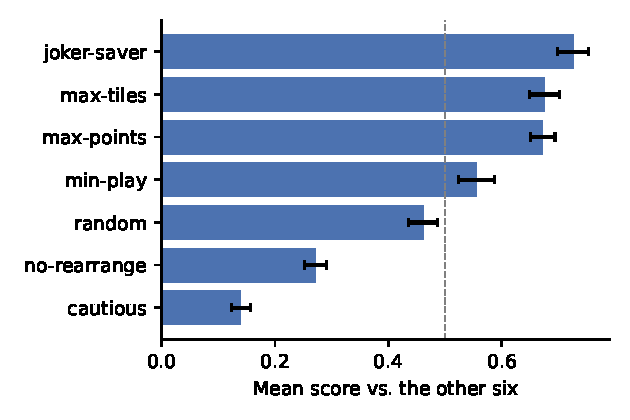
\includegraphics[width=\linewidth]{figuras/ranking.pdf}\caption{Ranking.}\label{fig:rank}\end{subfigure}
\begin{subfigure}{0.51\linewidth}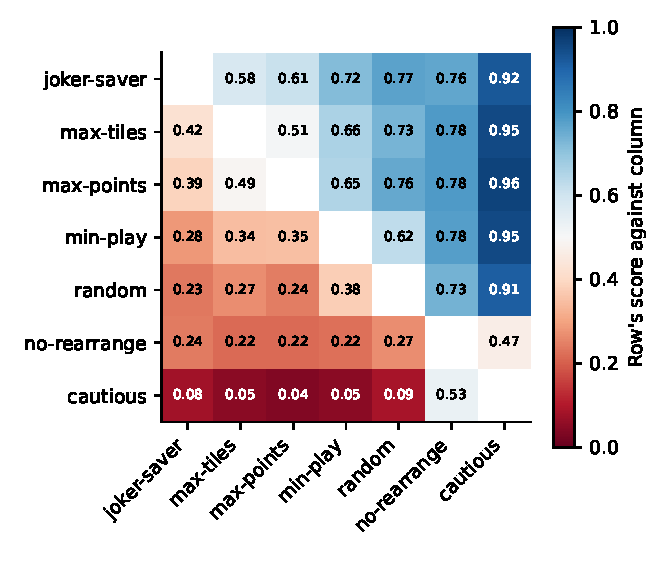
\includegraphics[width=\linewidth]{figuras/matriz.pdf}\caption{Head-to-head matrix.}\label{fig:matrix}\end{subfigure}
\caption{Paired round-robin (3{,}360 games); score: win $=1$, draw $=0.5$.}
\end{figure}

\subsection{RQ2: why does the joker-saver win?}\label{sec:mech}
The joker-saver differs from max-tiles in a single respect, how it treats jokers, so the question is which part of that behaviour matters. We state four candidate explanations and what each predicts. All comparisons are against max-tiles as opponent.
\begin{description}\itemsep0pt
\item[E1: a mild preference for spending fewer jokers.] Predicts that a soft penalty $\lambda$ per joker in the move score (maximising $n_{\text{tiles}}-\lambda n_{\text{jokers}}$) reproduces the gain.
\item[E2: recycling jokers on the table.] Rearranging lets a player take a joker out of a meld; saving jokers might make them less exposed to such steals. Predicts that forbidding the removal of a joker from its table meld removes the gain.
\item[E3: timing.] Predicts that sparing jokers only before the opening, or only after, isolates where the gain arises.
\item[E4: the joker as a finishing tile.] A joker completes almost any set, so holding one may make going out possible. Predicts that forbidding the joker even for the last move removes (and reverses) the gain, and that most wins of the saver end with a joker.
\end{description}
\begin{table}[h]\centering\small\setlength{\tabcolsep}{4pt}
\caption{Mechanism experiments: score of each variant against max-tiles (500 seeds $\times$ 2 seatings per row; the frozen max-tiles control is omitted), Holm-adjusted $p$ for mean $=0.5$, jokers played per game by the variant, jokers still in hand at the end of the game, and share of the variant's wins in which the final move used a joker. $\lambda>0$ penalises jokers, $\lambda<0$ rewards them.}\label{tab:mec}
\begin{tabular}{@{}lcrccc@{}}\toprule
Variant & Score & $p_{\text{Holm}}$ & Jokers played & Jokers left & Win with joker\\\midrule
joker-saver (full rule) & $0.568\pm0.027$ & $<0.001$ & 0.51 & 0.31 & 71\% \\
joker-saver, jokers frozen on table & $0.581\pm0.027$ & $<0.001$ & 0.53 & 0.32 & 75\% \\
save only after the opening meld & $0.537\pm0.022$ & 0.010 & 0.63 & 0.17 & 52\% \\
save only before the opening meld & $0.495\pm0.021$ & 1.000 & 0.77 & 0.01 & 5\% \\
never play a joker, even to go out & $0.189\pm0.021$ & $<0.001$ & 0.00 & 0.86 & 0\% \\
soft penalty $\lambda=4$ & $0.508\pm0.014$ & 1.000 & 0.77 & 0.01 & 6\% \\
soft penalty $\lambda=2$ & $0.506\pm0.006$ & 0.514 & 0.78 & 0.01 & 6\% \\
soft penalty $\lambda=1$ & $0.503\pm0.003$ & 0.661 & 0.78 & 0.01 & 4\% \\
soft penalty $\lambda=0.5$ & $0.500\pm0.000$ & 1.000 & 0.78 & 0.01 & 4\% \\
joker bonus $\lambda=-1$ & $0.500\pm0.000$ & 1.000 & 0.78 & 0.01 & 4\% \\
joker bonus $\lambda=-2$ & $0.500\pm0.000$ & 1.000 & 0.78 & 0.01 & 4\% \\
max-tiles mirror (control) & $0.500\pm0.000$ & 1.000 & 0.78 & 0.01 & 4\% \\
\bottomrule
\end{tabular}

\end{table}
\begin{figure}[h]\centering
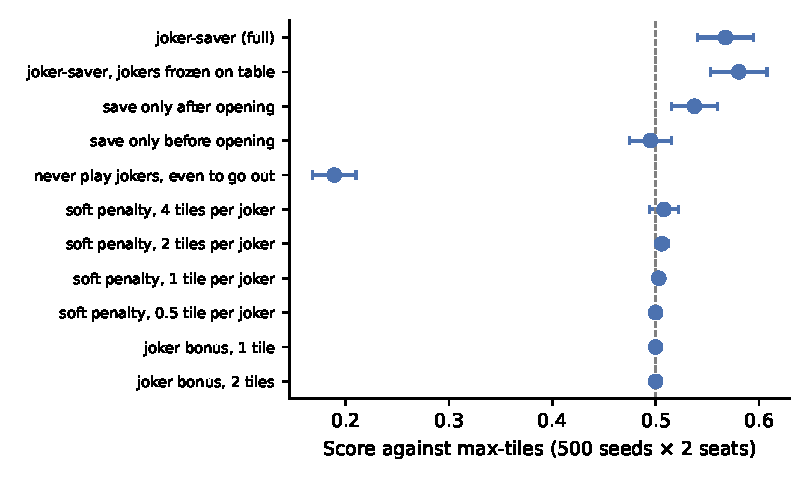
\includegraphics[width=0.75\linewidth]{figuras/dose_resposta.pdf}
\caption{Mechanism experiments (mean $\pm$ 95\% CI).}\label{fig:mec}
\end{figure}

\paragraph{E1 is not supported.} Soft penalties of $0.5$--$4$ tiles per joker give scores of $0.500$--$0.508$, none distinguishable from $0.5$ after correction, and a joker \emph{bonus} is identical to the control. The reason is visible in Table~\ref{tab:mec}: with soft penalties the player still spends $0.77$ jokers per game, as often as the control ($0.78$); a preference only breaks ties between moves of equal size. The saver's behaviour is qualitatively different: it \emph{refuses} to play joker moves and draws instead, keeping $0.31$ jokers in hand at the end of an average game.
\paragraph{E2 is not supported.} When jokers can never be removed from table melds, the saver's score is $0.581\pm0.027$, not lower than in the standard rules ($0.568\pm0.027$). The saver does not owe its edge to joker recycling or table theft.
\paragraph{E3: the effect arises after the opening.} Saving jokers only before the opening gives nothing ($0.495\pm0.021$); saving only after it gives $0.537\pm0.022$ ($p_{\text{Holm}}=0.01$). The two timings do not add up to the full rule ($0.568$), so part of the effect depends on both phases acting together; we have not isolated it.
\paragraph{E4 is supported.} If the saver is forbidden to use a joker even to empty its hand, its score collapses to $0.189\pm0.021$: it ends games holding $0.86$ jokers on average and never wins by going out with one. Conversely, $71\%$ of the full saver's wins end with a joker in the final move (against $4\%$ for max-tiles). Saving jokers is therefore \emph{only} beneficial when paired with spending them to go out. Because the full-rule and never-play variants differ \emph{only} in that exception, this is a within-simulator causal test (an intervention on the policy), not just a correlation.

\paragraph{Explanation.} The joker is a wildcard; spent early it saves a tile's worth of play, but held it keeps the hand completable. A hand that has been reduced to a few awkward tiles can often be finished only with a wildcard, so the saver trades a little early progress for the ability to finish when the opportunity arises. This is our interpretation of E3--E4; it is consistent with the interventions, but we did not test the narrower claim about ``awkward last tiles''.

\subsection{Sensitivity to the end-of-game rule}\label{sec:tie}
When the pool is empty and both players pass, the official rule awards the game to the player whose remaining tiles are worth the fewest points (a joker counts $30$). The main experiments score these games as draws ($16.3\%$ of the tournament). We replayed the same $3{,}360$ tournament games (same seeds) under the official rule and under a second one, fewest tiles in hand, and replayed the two ablations that matter most for E4 (500 seeds $\times$ 2 seatings each). Table~\ref{tab:tie} gives the results; Spearman's rank correlation of the seven-strategy ranking with the draw-rule ranking is $0.96$ for both alternatives.
\begin{table}[h]\centering\small
\caption{Tournament score (95\% CI) under three end-of-game rules. The last two rows are mechanism ablations against max-tiles. Fewest points is the official rule.}\label{tab:tie}
\begin{tabular}{@{}lccc@{}}\toprule
Strategy & Draw (0.5) & Fewest points & Fewest tiles\\\midrule
joker-saver & $0.726\pm0.027$ & $0.755\pm0.027$ & $0.765\pm0.027$ \\
max-tiles & $0.676\pm0.026$ & $0.713\pm0.025$ & $0.713\pm0.026$ \\
max-points & $0.672\pm0.022$ & $0.710\pm0.021$ & $0.710\pm0.021$ \\
min-play & $0.555\pm0.032$ & $0.594\pm0.030$ & $0.594\pm0.030$ \\
random & $0.461\pm0.026$ & $0.509\pm0.026$ & $0.509\pm0.026$ \\
cautious & $0.140\pm0.017$ & $0.208\pm0.018$ & $0.208\pm0.017$ \\
no-rearrange & $0.271\pm0.019$ & $0.010\pm0.006$ & $0.001\pm0.001$ \\
\midrule
Draws (\% of games) & 16.3 & 0.0 & 0.1 \\
Joker-saver vs.\ max-tiles & $0.568\pm0.027$ & $0.561\pm0.028$ & $0.561\pm0.028$ \\
Never-play-joker vs.\ max-tiles & $0.189\pm0.021$ & $0.164\pm0.021$ & $0.166\pm0.021$ \\
\bottomrule
\end{tabular}

\end{table}
The top of the ranking and the mechanism do not depend on the rule. The joker-saver stays first and its lead grows ($0.726\to0.755$ and $0.765$); max-tiles, max-points, min-play and random keep their order; head-to-head, the saver beats max-tiles by $0.561\pm0.028$ (official rule; $0.568$ under the draw rule), and forbidding the joker even for the last move still collapses it ($0.164\pm0.021$; $0.189$ under the draw rule). Fewest points and fewest tiles are almost indistinguishable ($0.0\%$ and $0.1\%$ of games remain tied), so the choice between them does not matter here. The only reordering is at the bottom: no-rearrange falls from $0.271$ to $0.010$ and below cautious. Its previous score was mostly pool-exhaustion draws: $54\%$ of its games ended that way, against $1.1\%$ of the other games, because a player that never touches the table seldom finishes. The official rule turns those stalemates into losses, so \emph{the draw rule flattered the weakest strategy and accounts for most of the $16.3\%$ draws}. The Jev-meta results were obtained under the draw rule and were not repeated; Q-meta was retrained and re-evaluated under the official rule (Section~\ref{sec:rlrule}).

\subsection{Sensitivity to the rearrangement search cap}\label{sec:cap}
The simulator lists rearrangements by a bounded search: at most $128$ plans, $1{,}000$ search visits, $2$ table sets and $18$ tiles per rearrangement. Instrumenting the search shows that the $128$-plan cap is reached in $9.9\%$ of decisions and in $73\%$ of tournament games, so the cap is not harmless. We therefore replayed the tournament (7 strategies, 21 pairs, 40 seeds, both seats, official end-of-game rule) with larger caps: $\times4$ ($512$ plans), $\times16$ ($2{,}048$) and a large profile ($4{,}096$ plans, $3$ sets, $24$ tiles). Games are paired by pair, seed and seat. The no-rearrange\,/\,cautious pair was dropped from all columns because $47$ of its $80$ large-profile games had not finished when we stopped the run, so all columns use the same $1{,}600$ games.
\begin{table}[h]\centering\small\setlength{\tabcolsep}{4pt}
\caption{Tournament score by rearrangement cap (plans per decision). The last row is joker-saver vs.\ max-tiles with a bootstrap $95\%$ interval over $40$ seeds.}\label{tab:cap}
\begin{tabular}{@{}lcccc@{}}\toprule
Strategy & Default (128) & $\times4$ (512) & $\times16$ (2048) & Large (4096)\\\midrule
joker-saver & $0.690$ & $0.729$ & $0.736$ & $0.783$ \\
max-tiles & $0.685$ & $0.681$ & $0.680$ & $0.698$ \\
max-points & $0.662$ & $0.648$ & $0.647$ & $0.680$ \\
min-play & $0.596$ & $0.568$ & $0.564$ & $0.592$ \\
random & $0.486$ & $0.484$ & $0.482$ & $0.520$ \\
no-rearrange & $0.217$ & $0.220$ & $0.219$ & $0.045$ \\
cautious & $0.039$ & $0.048$ & $0.050$ & $0.028$ \\
\midrule
Decisions at the plan cap (\%) & 9.9 & 1.6 & 0.1 & 0.4 \\
Joker-saver vs.\ max-tiles & $0.525$ [0.42, 0.62] & $0.556$ [0.45, 0.66] & $0.562$ [0.46, 0.66] & $0.625$ [0.53, 0.72] \\
\bottomrule\end{tabular}

\end{table}
\begin{figure}[h]\centering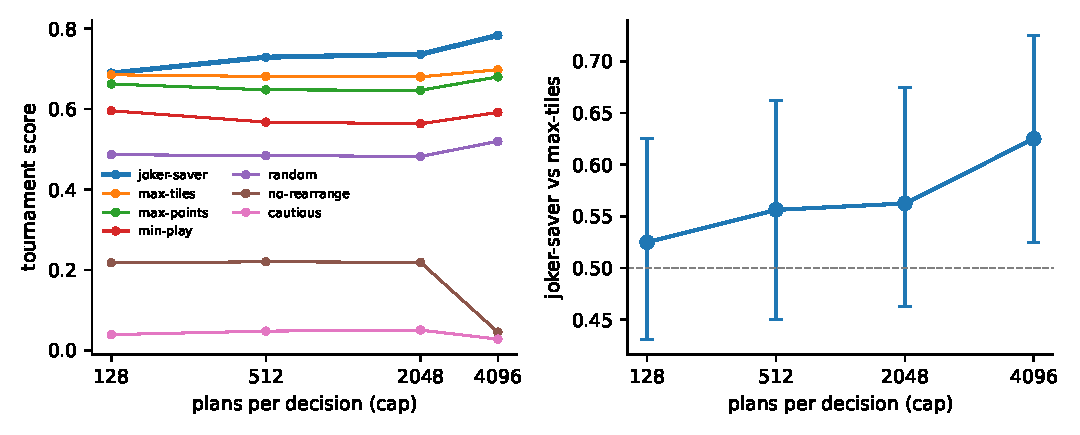
\includegraphics[width=\linewidth]{figuras/limites.pdf}
\caption{Left: tournament score of each strategy by rearrangement cap. Right: joker-saver against max-tiles with the $95\%$ bootstrap interval over $40$ seeds.}\label{fig:cap}\end{figure}
The ranking is identical in the four columns (Table~\ref{tab:cap}, Figure~\ref{fig:cap}), and the joker-saver's advantage grows with the cap ($0.525\to0.556\to0.562\to0.625$ head-to-head over max-tiles), so truncation does not explain the result and, if anything, understates it. The head-to-head interval at the default cap includes $0.5$ with only $40$ seeds (the main tournament has more); the large-profile interval does not, but this comparison is exploratory. The collapse of no-rearrange in the large profile ($0.217\to0.045$) is consistent with opponents that rearrange finishing earlier (mean $99.5$ vs.\ $111.9$ decisions in its games); we did not test this further. An offline oracle re-enumerated $383$ capped states with the large profile: it found a play with more tiles in $4.2\%$ of them, always by exactly one tile ($0.3\%$ with $\times4$). Jev, PIMC and the move network were not rerun with larger caps.

\subsection{Beyond two players}\label{sec:mesa}
The simulator accepts up to ten players; this section uses three and four (pools of $64$ and $50$ tiles after the deal; games last about $71$ and $50$ decisions against $96$ for two players). The strategies of Table~\ref{tab:strat} do not look at opponents, so they run unchanged; the learned agents look at the opponents and were retrained for each table size (below); the Monte Carlo search was not rerun (Jev was, see the end of this subsection). One focus strategy plays all seats in rotation, so each seed gives $N$ games, and we score a win as $1$ and a draw as $1/N$, so the baseline is $1/N$. The opponents are either copies of max-tiles or a mixed field of $N-1$ distinct strategies drawn at random from the other six. Intervals are $\pm1.96$ standard errors over seeds. Each strategy has $100$ seeds; the joker-saver against max-tiles has $500$ (added after the first $100$ were inconclusive, so this comparison is a follow-up rather than a pre-specified one).
\begin{table}[h]\centering\small
\caption{Score of one focus strategy at three- and four-player tables (win $=1$; chance $=1/N$). ``vs max-tiles'': the other seats are max-tiles; max-tiles against itself is $1/N$ by symmetry. ``Mixed field'': other seats drawn at random among the six remaining strategies, so the field differs slightly between rows. The joker-saver's ``vs max-tiles'' cells use $500$ seeds, all other cells $100$. The two lower rows are learned agents trained for the table size: the network is the policy-gradient move network of Section~\ref{sec:moves} retrained at $N=3$ and $N=4$ (1{,}500 iterations; $100$ evaluation seeds per cell), the Q-learner is the strategy selector retrained with five replicas (20 evaluation seeds each; intervals over replica--seed pairs). The no-winner row pools all rows.}\label{tab:mesa}
\begin{tabular}{@{}lcccc@{}}\toprule
 & \multicolumn{2}{c}{3 players ($1/N=0.333$)} & \multicolumn{2}{c}{4 players ($1/N=0.250$)}\\
Strategy & vs max-tiles & mixed field & vs max-tiles & mixed field\\\midrule
joker-saver & $0.374\pm0.021$ & $0.567\pm0.061$ & $0.249\pm0.015$ & $0.378\pm0.041$ \\
max-tiles & $0.333\pm0.000$ & $0.536\pm0.060$ & $0.250\pm0.000$ & $0.421\pm0.049$ \\
max-points & $0.353\pm0.038$ & $0.470\pm0.060$ & $0.273\pm0.027$ & $0.416\pm0.054$ \\
min-play & $0.213\pm0.039$ & $0.412\pm0.067$ & $0.128\pm0.031$ & $0.246\pm0.039$ \\
random & $0.150\pm0.038$ & $0.267\pm0.055$ & $0.070\pm0.026$ & $0.139\pm0.038$ \\
cautious & $0.027\pm0.018$ & $0.063\pm0.026$ & $0.020\pm0.013$ & $0.024\pm0.014$ \\
no-rearrange & $0.008\pm0.006$ & $0.007\pm0.005$ & $0.003\pm0.002$ & $0.003\pm0.003$ \\
\midrule
network & $0.390\pm0.046$ & $0.477\pm0.057$ & $0.275\pm0.036$ & $0.404\pm0.044$ \\
Q-learner & $0.130\pm0.041$ & $0.272\pm0.052$ & $0.112\pm0.026$ & $0.176\pm0.040$ \\
\midrule
Games with no winner (\%) & 0.2 & 0.6 & 0.2 & 0.8 \\
\bottomrule\end{tabular}

\end{table}
\begin{figure}[h]\centering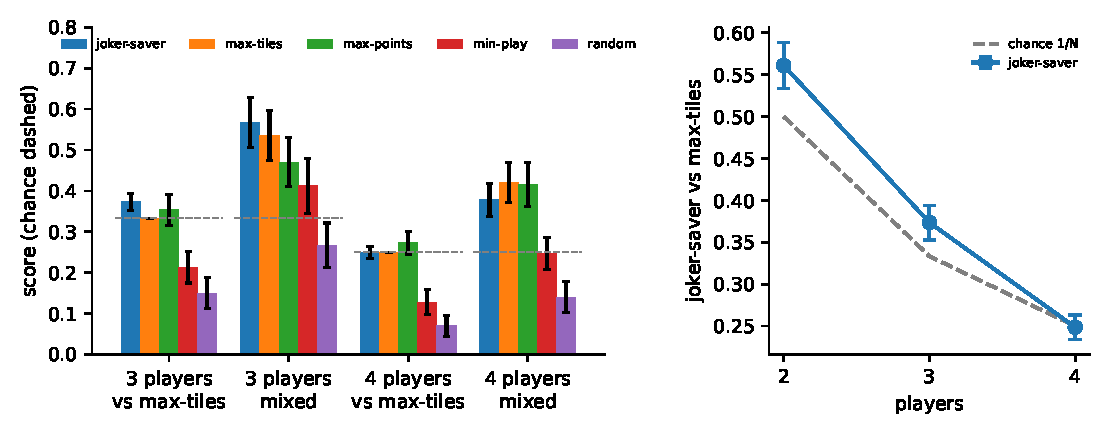
\includegraphics[width=\linewidth]{figuras/mesa.pdf}
\caption{Left: score of five strategies at three- and four-player tables (dashed: chance $1/N$). Right: joker-saver against max-tiles as the number of players grows ($\pm1.96$ standard errors over seeds).}\label{fig:mesa}\end{figure}
The lower half of the ranking is the same as with two players (Figure~\ref{fig:mesa}) (min-play, random, cautious and no-rearrange are far below chance). At the top, the picture changes. Against three max-tiles opponents at a four-player table the joker-saver scores $0.249\pm0.015$, exactly chance ($0.25$): its advantage disappears. At a three-player table it keeps a smaller advantage, $0.374\pm0.021$ against $0.333$. The same strategy forbidden from playing a joker even as its last move falls to $0.159\pm0.015$ at three players ($500$ seeds), as at two players ($0.164$), so the finishing-joker mechanism still holds where the advantage exists. In the mixed fields the top three strategies are not separable with $100$ seeds. We do not know why the advantage shrinks at four players; a plausible but untested reason is that games end sooner, leaving fewer turns in which holding a joker can pay. Games with no winner are rare ($0.1$--$0.7\%$). The learned agents behave differently from the heuristics. The tabular selector retrained at three and four players (five replicas, 1{,}200 training games each) ends \emph{below} chance in every cell (Table~\ref{tab:mesa}; $0.130\pm0.041$ and $0.112\pm0.026$ against max-tiles): its coarse state summarises the opponents by one number and does not carry over. The move network retrained for each table size is the first learned agent that is not below its reference: against max-tiles it scores $0.390\pm0.046$ at three players and $0.275\pm0.036$ at four, statistically indistinguishable from the joker-saver ($0.374\pm0.021$, $0.249\pm0.015$) at the same seeds, and only marginally above chance. In the mixed fields it is below the joker-saver at three players ($0.477\pm0.057$ against $0.567\pm0.061$) and level at four ($0.404\pm0.044$ against $0.378\pm0.041$). These are exploratory comparisons, with a single training run per table size and no multiplicity correction; we read them as ``no worse than the best heuristic once the field is crowded'', not as a win. A plausible but untested reading is that with more opponents the choice between drawing and playing matters less, which is also where the joker-saver's edge disappears. These are heuristic-versus-heuristic results, plus one training run of each learned agent.

\paragraph{Jev at three and four players.} We ran the strategy-selecting Jev agent (same prompt, with the opponents summarised by hand size and whether they have melded) at both table sizes: $80$ seeds, every seat, $1{,}680$ games, US\$1.43 in total. Against max-tiles opponents its result is identical to max-tiles in every game ($1/N$ exactly, $0.333$ and $0.250$). In a mixed field, on the same opponents as max-tiles and paired by seed, it scores $0.544\pm0.068$ and $0.398\pm0.052$, against $0.544$ and $0.401$ for max-tiles and $0.557\pm0.056$ and $0.426\pm0.048$ for the joker-saver (differences to max-tiles: $0.000$ and $-0.003\pm0.006$). The reason is visible in its choices: of $21{,}068$ answers, $19{,}029$ chose max-tiles (including $9{,}884$ low-confidence fallbacks to it), $2{,}039$ chose ``draw'' (when the other options draw as well) and one chose another strategy; it never selected the joker-saver. With more players Jev still behaves as max-tiles. The agent that chooses the concrete move (Jev-moves) was also run at both sizes, on $40$ seeds in the mixed field, paired with max-tiles on the same opponents ($280$ games, $3{,}251$ calls, no fallbacks, US\$0.37): it scores $0.567\pm0.108$ against $0.589\pm0.091$ for max-tiles at three players (difference $-0.022\pm0.095$) and $0.412\pm0.080$ against $0.408\pm0.081$ at four ($+0.005\pm0.086$), with the joker-saver at $0.603\pm0.074$ and $0.438\pm0.076$ on these seeds. It is indistinguishable from max-tiles at these table sizes, whereas against a single opponent it was clearly below it ($0.350\pm0.076$); the sample is small and we do not claim the difference between table sizes is real. Total spend on the Jev agents at the larger tables: US\$1.80.

\subsection{Stronger opponents: an extended league}\label{sec:liga}
The ranking above is relative to seven strategies we wrote. To see whether a more elaborate strategy displaces the joker-saver, we added five exploratory ones, defined before running and not tuned afterwards: \emph{adaptive} (joker-saver until some opponent has $\le4$ tiles, then max-tiles), \emph{reorganiser} (prefers moves that avoid spending jokers and that move jokers already on the table), \emph{flexible} (max-tiles, ties broken by the number of tile pairs left in hand that could still form a meld), and \emph{saver-until-$N$} ($N=2,3$: the joker-saver, but a joker may be spent once the hand has $N$ tiles or fewer). We ran a paired round robin of all $12$ strategies ($66$ pairs, $80$ new seeds, both seats, official end-of-game rule; $10{,}560$ games, none truncated). Strength is also summarised by a Bradley--Terry fit, with a draw counted as half a win.
\begin{table}[h]\centering\small
\caption{Extended league ($^*$: exploratory strategy). Mean score over the other eleven strategies, Bradley--Terry strength, and the share of the strategy's wins that ended with a joker, measured only in games where it occupies the first slot of the pair (saver-until-$3$ never does).}\label{tab:liga}
\begin{tabular}{@{}lccc@{}}\toprule
Strategy & Mean score & Bradley--Terry & Wins ending with a joker (\%)\\\midrule
joker-saver & $0.652$ & $2.64$ & 59 \\
saver-until-2* & $0.641$ & $2.51$ & 62 \\
saver-until-3* & $0.628$ & $2.38$ & -- \\
flexible* & $0.624$ & $2.33$ & 8 \\
adaptive* & $0.620$ & $2.29$ & 18 \\
max-points & $0.602$ & $2.11$ & 5 \\
max-tiles & $0.593$ & $2.03$ & 4 \\
reorganiser* & $0.542$ & $1.62$ & 5 \\
min-play & $0.531$ & $1.55$ & 0 \\
random & $0.418$ & $0.92$ & 0 \\
cautious & $0.136$ & $0.12$ & 2 \\
no-rearrange & $0.013$ & $0.01$ & 0 \\
\bottomrule\end{tabular}

\end{table}
\begin{figure}[h]\centering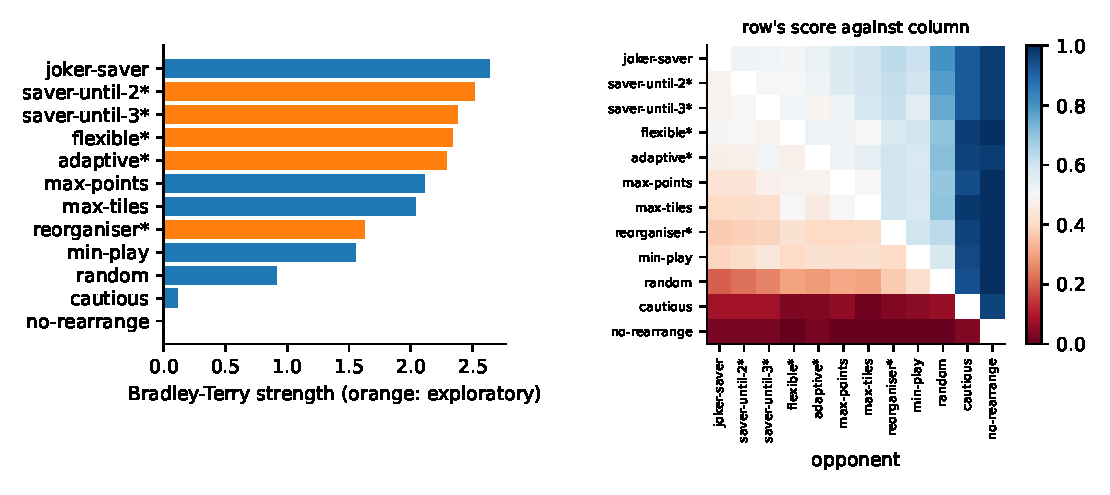
\includegraphics[width=\linewidth]{figuras/liga.pdf}
\caption{Extended league. Left: Bradley--Terry strength (orange: exploratory strategies). Right: score of the row strategy against the column strategy ($80$ seeds, both seats).}\label{fig:liga}\end{figure}
The joker-saver stays first by mean score and Bradley--Terry strength (Figure~\ref{fig:liga}), but the three variants that keep a joker until the end (joker-saver, saver-until-$2$, saver-until-$3$) are not separable here: joker-saver against saver-until-$2$ is $0.519$ ($p=0.08$). Head-to-head against max-tiles the joker-saver scores $0.600\pm0.075$ ($p=0.009$), but with $66$ comparisons this does not survive the Holm correction, so the original result (more seeds, Section~\ref{sec:protocol}) remains the confirmatory one. Among the eight strongest strategies the only pairs significant after Holm involve the reorganiser, which loses to the joker-saver ($0.369\pm0.071$) and to both saver-until variants: moving table jokers instead of playing more tiles does not pay. Adaptive ($0.544\pm0.068$ against max-tiles) and flexible ($0.500\pm0.068$) are not distinguishable from max-tiles or from the joker-saver. Of the $32$ pairs that are significant after Holm, none forms a three-way cycle, so strength is transitive on this menu. The finishing-joker pattern reappears: $59$--$62\%$ of the wins of the joker-saver and of saver-until-$2$ end with a joker, against $0$--$18\%$ for the others. None of the new strategies is better than the joker-saver at this sample size; this does not show that none could be, nor does it say anything about human play.

\subsection{Jokers in hand: initial deal and draws}
\label{sec:ini}
How much is a joker in the initial hand worth? We played $2{,}000$ \emph{mirror} games (both seats use the same strategy; seeds $50000$ and up) for random, max-tiles and joker-saver and grouped the $4{,}000$ initial hands per strategy by the number of jokers they contain (Table~\ref{tab:ini}, Figure~\ref{fig:ini}). Each entry is the mean score of hands with that number of jokers; the two hands of a game are counted separately and treated as independent in the intervals, an approximation we did not check.
\begin{table}[h]\centering\small
\caption{Mean score of an initial hand by number of jokers, mirror matches (95\% CI; number of hands in parentheses).}\label{tab:ini}
\begin{tabular}{@{}lccc@{}}\toprule
Strategy (mirror) & 0 jokers & 1 joker & 2 jokers\\\midrule
max-tiles & 0.497$\pm$0.018 (3025) & 0.507$\pm$0.033 (903) & 0.542$\pm$0.116 (72) \\
joker-saver & 0.466$\pm$0.018 (3025) & 0.600$\pm$0.031 (903) & 0.674$\pm$0.103 (72) \\
random & 0.504$\pm$0.018 (3025) & 0.494$\pm$0.033 (903) & 0.403$\pm$0.114 (72) \\
\bottomrule
\end{tabular}

\end{table}
\begin{figure}[h]\centering
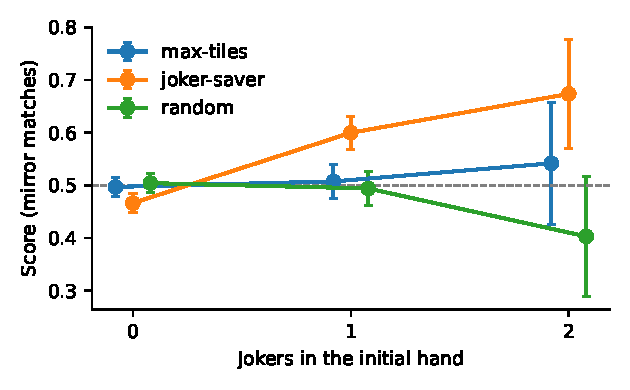
\includegraphics[width=0.5\linewidth]{figuras/coringas_iniciais.pdf}
\caption{Score by number of initial jokers, mirror matches.}\label{fig:ini}
\end{figure}
A joker in the opening hand is worth a substantial edge \emph{only for the joker-saver}: with one joker it scores $0.600\pm0.031$ and with two $0.674\pm0.103$ (72 hands only, so the interval is wide), against $0.466\pm0.018$ with none. Under max-tiles the score is $0.497$, $0.507\pm0.033$ and $0.542\pm0.116$, and under random $0.504$, $0.494\pm0.033$ and $0.403\pm0.114$, so a joker confers no detectable advantage to a player that does not hold it for the final move. This agrees with Section~\ref{sec:mech} (E4): the value of a joker depends on the policy that uses it. The two-joker estimate is imprecise and should not be read as a precise win probability.

\paragraph{Pooled field.} The mirror design covers only three strategies. To ask the question without fixing the strategy, we played $4{,}000$ games ($2{,}000$ seeds $\times$ 2 seatings, seeds $90000$ and up, official tie-break) in which each seed assigns one of the $28$ pairings, with repetition, of the seven strategies, and pooled the $8{,}000$ hands. Intervals resample seeds. Table~\ref{tab:campo} gives the result. A hand without an initial joker scores $0.496\pm0.006$, with one $0.509\pm0.020$, with two $0.576\pm0.081$ ($118$ hands): averaged over the field, a starting joker is worth about one or two points, and the interval for one joker contains $0.5$. Comparing, within each strategy, hands with and without a starting joker gives $+0.025$ [$0.000$, $0.052$].

\paragraph{Jokers drawn from the pool.} A joker can also arrive by drawing. Each player chooses to draw $29.7$ times per game on average (draws after the pool is empty are passes), so most of the $78$-tile pool is drawn: $50\%$ of hands ($3{,}991$ of $8{,}000$) draw at least one joker ($0.59$ per hand). A naive comparison is misleading: hands that drew a joker score $-0.015$ [$-0.043$, $0.012$] relative to those that did not, because players who draw more are usually behind and, drawing more, meet more jokers. We therefore compare hands within strata of the number of draws (five groups cut at the quintiles $23$, $27$, $31$, $38$; the pooled estimate uses strategy $\times$ quintile cells, the per-strategy estimates use the quintiles within each strategy), averaging the stratum differences with weights $n_1n_0/(n_1+n_0)$. The adjusted difference is $+0.037$ [$0.012$, $0.064$]. Figure~\ref{fig:comprado} shows the estimate per strategy: only the joker-saver has a clearly positive effect ($+0.119$ [$0.055$, $0.186$]), followed by max-points ($+0.081$ [$0.017$, $0.151$]) and max-tiles ($+0.053$ [$-0.015$, $0.120$]); random, cautious, min-play and no-rearrange are indistinguishable from zero. The joker-saver's drawn-joker effect agrees with its mirror-match initial-joker effect ($+0.13$). In the pooled field, however, the joker-saver's \emph{initial}-joker difference is $0.003$ ($0.681\pm0.066$ with one or more, $0.678\pm0.030$ with none; $251$ hands), about three standard errors below the mirror estimate; we did not find a reason, and note it as an open point (the opponent in the mirror also saves jokers for the last move, which may matter).
\begin{table}[h]\centering\small
\caption{Pooled field (seven strategies, $8{,}000$ hands): mean score by number of initial and drawn jokers, and effect of having a joker (hands with $\ge1$ minus hands with none). Intervals: normal over seeds for the group means; bootstrap over seeds for the effects. Bracketed values are 95\% intervals.}\label{tab:campo}
\begin{tabular}{@{}lcr@{}}\toprule
Group & Score (pooled field) & Hands\\\midrule
Initial jokers = 0 & 0.496$\pm$0.006 & 6068 \\
Initial jokers = 1 & 0.509$\pm$0.020 & 1814 \\
Initial jokers = 2 & 0.576$\pm$0.081 & 118 \\
\midrule
Bought jokers = 0 & 0.508$\pm$0.014 & 4009 \\
Bought jokers = 1 & 0.498$\pm$0.015 & 3282 \\
Bought jokers = 2 & 0.468$\pm$0.042 & 709 \\
\midrule
Initial joker, effect (strategy-stratified) & \multicolumn{2}{c}{$+0.025$ [+0.000, +0.052]} \\
Bought joker, naive difference & \multicolumn{2}{c}{$-0.015$ [-0.043, +0.011]} \\
Bought joker, stratified by draws & \multicolumn{2}{c}{$+0.037$ [+0.012, +0.064]} \\
\bottomrule
\end{tabular}

\end{table}
\begin{figure}[h]\centering
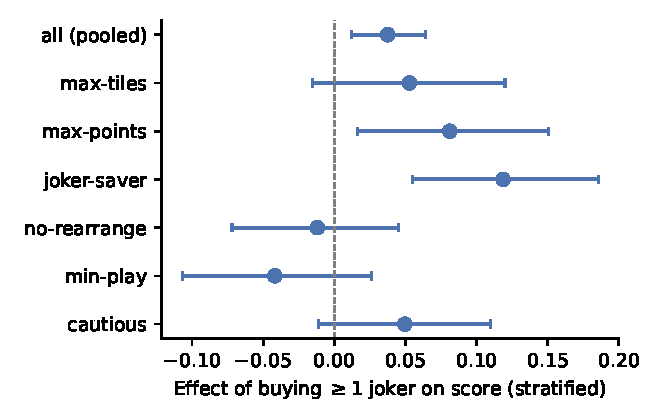
\includegraphics[width=0.55\linewidth]{figuras/coringa_comprado.pdf}
\caption{Effect of drawing at least one joker on the score, within strata of the number of draws, by strategy (95\% bootstrap intervals).}\label{fig:comprado}
\end{figure}
Both routes lead to the same conclusion as Section~\ref{sec:mech}: a joker is worth little to a player who spends it as soon as it helps, and its value is realised by the strategy that holds it for the last move. Because the player cannot choose when a joker arrives, this is a statement about the policy, not about the tile.


\subsection{RQ3a: Q-learning over strategies}
The moving-average training score rises from $0.50$ (first 100 games) to $0.61$ (last 100), averaged over five replicas (Figure~\ref{fig:learn}). Against the field the greedy policy scores $0.62\pm0.05$, but this is dominated by weak opponents (Figure~\ref{fig:rlvs}): against the best heuristics it scores $0.42\pm0.07$ (joker-saver), $0.47$ (max-tiles) and $0.47$ (max-points), with intervals including $0.5$ for the latter two, and against random $0.675\pm0.081$, a point estimate below that of the fixed max-tiles ($0.731$) and joker-saver ($0.766$) against random, though the intervals overlap. The learned policy therefore does not exceed the best fixed strategy. This is consistent with the coarse state, a sparse terminal reward and only $1{,}200$ episodes per replica; we cannot say whether more training or a richer state would change the conclusion. The learned policies are diffuse (Figure~\ref{fig:policy}), so we make no claim about when to switch strategy.
\begin{figure}[h]\centering
\begin{subfigure}{0.48\linewidth}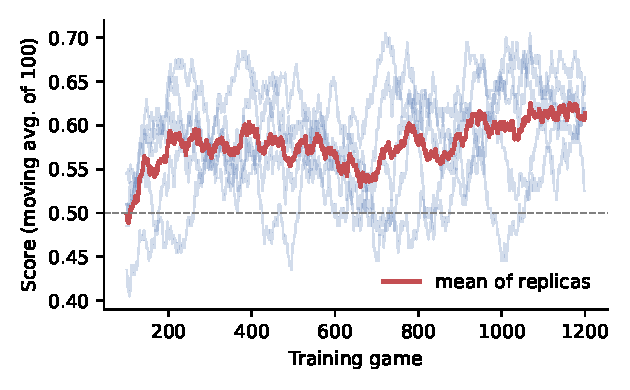
\includegraphics[width=\linewidth]{figuras/aprendizado.pdf}\caption{Learning curve.}\label{fig:learn}\end{subfigure}
\begin{subfigure}{0.48\linewidth}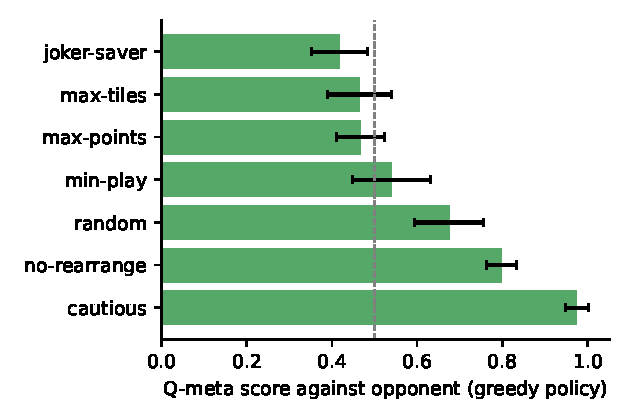
\includegraphics[width=\linewidth]{figuras/rl_vs_oponentes.pdf}\caption{Q-meta against each opponent.}\label{fig:rlvs}\end{subfigure}
\caption{Q-meta training and evaluation (5 replicas).}
\end{figure}
\begin{figure}[h]\centering
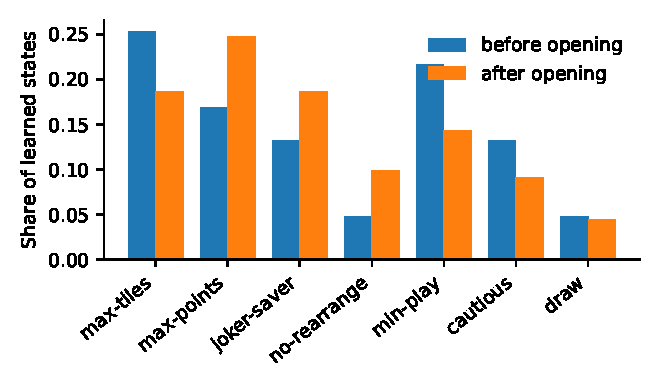
\includegraphics[width=0.5\linewidth]{figuras/politica.pdf}
\caption{Share of learned states where each strategy has the highest Q-value, by opening status.}\label{fig:policy}
\end{figure}

\subsection{RQ3b: Jev as a strategy selector}
Over 600 games Jev made 28{,}090 calls (29.2M input tokens, US\$1.23 at US\$0.042 per million tokens; output is free; 7 transport failures). In $49\%$ of calls confidence fell below $0.3$ and the fallback (max-tiles) was used; of the 14{,}237 answered decisions, $84\%$ chose max-tiles and $16\%$ ``draw''; the other options were essentially never chosen (Figure~\ref{fig:jev}). It scores $0.50$ against max-tiles, $0.68\pm0.06$ against random and $0.40\pm0.06$ against joker-saver: in this protocol it behaves like max-tiles and misses the joker-saver's mechanism (E4), which its prompt did not describe. The sample is small and exploratory, with one prompt and one model version.
\begin{figure}[h]\centering
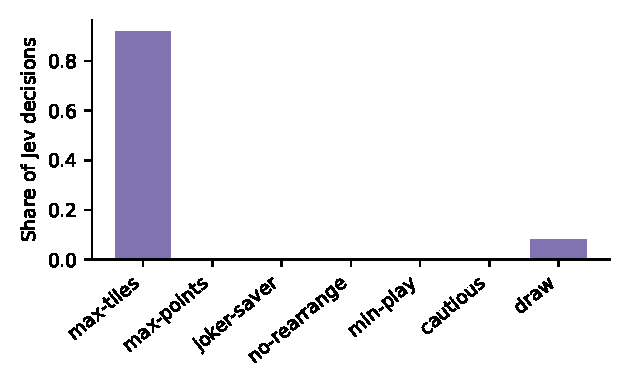
\includegraphics[width=0.45\linewidth]{figuras/jev_escolhas.pdf}
\caption{Distribution of Jev's choices (including fallbacks).}\label{fig:jev}
\end{figure}

\subsection{Q-meta under the official end-of-game rule}\label{sec:rlrule}
We retrained the five Q-meta replicas ($1{,}200$ games each) and re-evaluated them with fewest points deciding a stalled pool. Scores (100 seed pairs per opponent, pooled over replicas; the interval ignores clustering by replica and is therefore optimistic) are below; the draw-rule values from the previous subsection are in brackets.
\begin{center}\small
\begin{tabular}{lcc}
\toprule
Opponent & Official rule & [Draw rule]\\
\midrule
joker-saver & $0.370\pm0.060$ & [$0.417\pm0.072$]\\
max-tiles & $0.410\pm0.066$ & [$0.465\pm0.063$]\\
random & $0.595\pm0.062$ & [$0.675\pm0.058$]\\
mean over the seven opponents & $0.616\pm0.027$ & [$0.620\pm0.026$]\\
\bottomrule
\end{tabular}
\end{center}
The conclusion is unchanged: the learned selector remains below the joker-saver and max-tiles, and the field average is dominated by weak opponents. Part of the draw-rule score against the strong heuristics came from stalled-pool draws.

\subsection{RQ3c: agents that choose the move}\label{sec:moves}
The three agents below were evaluated under the official rule, paired by seed with alternating seats.
\begin{table}[h]\centering\small
\caption{Move-choosing agents against fixed heuristics (score $\pm$ 95\% CI over seeds; $p$ for mean $=0.5$, uncorrected).}\label{tab:moves}
\begin{tabular}{llccc}
\toprule
Agent & Opponent & Seeds & Score & $p$\\
\midrule
Jev-moves & max-tiles & 70 & $0.350\pm0.076$ & $<0.001$\\
Jev-moves & joker-saver & 70 & $0.414\pm0.072$ & $0.019$\\
PIMC $D{=}4$ & max-tiles & 60 & $0.542\pm0.091$ & $0.37$\\
PIMC $D{=}4$ & joker-saver & 60 & $0.433\pm0.085$ & $0.13$\\
PIMC $D{=}2$ & joker-saver & 30 & $0.267\pm0.122$ & $<0.001$\\
PIMC $D{=}8$ & joker-saver & 30 & $0.400\pm0.128$ & $0.13$\\
Move network & joker-saver & 500 & $0.403\pm0.030$ & $<0.001$\\
Move network & max-tiles & 500 & $0.493\pm0.029$ & $0.63$\\
Move network & max-points & 500 & $0.492\pm0.029$ & $0.59$\\
Move network & min-play & 500 & $0.634\pm0.029$ & $<0.001$\\
Move network & random & 500 & $0.732\pm0.027$ & $<0.001$\\
\bottomrule
\end{tabular}
\end{table}
\paragraph{Jev-moves.} Over 280 games Jev answered about $6{,}000$ decisions (about $2{,}000$ input tokens per call, US\$0.0018 per game, US\$0.51 in total); the fallback was used $7$ times. Its mean confidence was $0.38$, low as expected with about $30$ options. Its choice coincided with max-tiles' choice in $40\%$ of decisions, it drew in $3\%$ and played a joker in only $3$--$4\%$, so it neither reproduces the biggest-move rule nor the finishing-joker rule. It is clearly worse than max-tiles and worse than the joker-saver. The prompt gave the rules and the consequence of every option but no strategy advice; other prompts (for instance one that stresses emptying the hand) were not tried.
\paragraph{PIMC.} With $D=4$ worlds the search is statistically indistinguishable from max-tiles ($0.542$) and from the joker-saver ($0.433$, whose interval includes $0.5$), but with $60$ seeds the power is low. More worlds did not help ($D=8$: $0.400$) and fewer clearly hurt ($D=2$: $0.267$). The cost is about $105$\,s per game for $D=4$ against about $1.3$\,s for a heuristic. Because the rollout policy is itself the joker-saver, the search can at best correct its choices at the margin, and ties are resolved in its favour; we therefore read this as ``search with this rollout does not beat the joker-saver'', not as a bound on search in general.

\paragraph{Move network.} To remove the strategy menu from the learner we trained a small policy that scores each legal move directly: a network with $15$ features per move (move size, jokers used, hand and pool sizes, opening status, \dots), one hidden layer of $16$ tanh units and a softmax over the legal moves, written in plain Python. It was trained by REINFORCE with an exponential-moving-average baseline, Adam ($3{\times}10^{-3}$) and an entropy bonus ($0.01$) for $1{,}500$ iterations of $24$ games ($36{,}000$ games), with reward $\pm1$ at the end of the game. Opponents were drawn from a league: $50\%$ the seven heuristics, $25\%$ the current network, $25\%$ one of its last ten snapshots. It is evaluated greedily on $500$ held-out seeds per opponent, both seatings ($7{,}000$ games, none truncated). It plays like max-tiles: $0.493$ and $0.492$ against max-tiles and max-points (both intervals include $0.5$), where max-tiles itself scores $0.506$ against max-points. It beats the weaker heuristics by about as much as max-tiles does ($0.732$ against random, where max-tiles scores $0.731$; $0.634$ against min-play, $0.656$). Against the joker-saver it scores $0.403\pm0.030$, below $0.5$ and close to what max-tiles obtains ($0.425$ in the tournament, $80$ seeds). The finishing-joker rule was not learned: it went out with a joker in $2.9\%$ of games (max-tiles $3.5\%$, joker-saver $41\%$) and played $0.80$ jokers per game (max-tiles $0.83$). The training-time win rate against heuristics rose slowly from $0.59$ to $0.64$ (blocks of $250$ iterations); it is measured on a changing league and is not evidence of strength. This is one run of one architecture and one learning rate, with no hyper-parameter search, so we read it as ``this learner, with this budget, converges to max-tiles-like play'' and not as a limit of reinforcement learning.

\paragraph{Starting from imitation (exploratory).} Because the network trained from scratch never found the finishing-joker rule, we first asked whether the features can represent it at all. We cloned the joker-saver by supervised learning on $10{,}587$ of its decisions (300 games against the seven heuristics, with rearrangement; the same likelihood as REINFORCE with advantage $1$). The clone agrees with the saver's choice in $82\%$ of held-out decisions, goes out with a joker in $70\%$ of its wins against the saver ($71\%$ for the saver itself) and scores $0.43\pm0.07$ against the saver and $0.485\pm0.07$ against max-tiles ($100$ seeds, seeds $160{,}000$ and up). So the $15$ features and one hidden layer suffice to represent the mechanism; what the from-scratch run lacked was the search for it. We then ran the same REINFORCE for $300$ iterations from the clone (learning rate $3\times10^{-3}$, fixed before the replication). On the first training seed this scored $0.545\pm0.07$ against the saver and $0.605\pm0.07$ against max-tiles, the only result in this paper that seemed to beat both. We replicated it with two further training seeds and evaluated all three on fresh seeds ($170{,}000$ and up, $80$ pairs each, Table~\ref{tab:clone}). The replication does not confirm the first number: pooled over the three trainings the agent scores $0.509\pm0.045$ against max-tiles and $0.487\pm0.045$ against the saver, so it ties with both. The first score was a favourable draw of seeds and training run (selection of the best of several looks). The agent's use of jokers also varies across trainings (going out with a joker in $41\%$, $17\%$ and $41\%$ of wins), so imitation did not fix the mechanism in a stable way. The substantive change is against the saver, where the from-scratch network scored $0.403\pm0.030$ ($500$ games) and the cloned-then-trained agent $0.487\pm0.045$ ($480$ games). Table~\ref{tab:clone} does not meet the criterion we had set for a positive result (an interval excluding $0.5$ against max-tiles).
\begin{table}[h]\centering\small
\caption{Confirmatory evaluation of the network started from the clone of the joker-saver and then trained by REINFORCE ($300$ iterations), three training seeds, seeds $170{,}000$+, $160$ games each; $\pm$ is the 95\% CI over games.}\label{tab:clone}
\begin{tabular}{lccc}\toprule
Training seed & vs max-tiles & vs joker-saver & Wins ending with a joker (vs max-tiles)\\\midrule
0 & $0.512\pm0.077$ & $0.475\pm0.077$ & $41\%$\\
1 & $0.484\pm0.077$ & $0.487\pm0.077$ & $17\%$\\
2 & $0.531\pm0.077$ & $0.500\pm0.077$ & $41\%$\\
Pooled ($480$ games) & $0.509\pm0.045$ & $0.487\pm0.045$ & \\
\bottomrule\end{tabular}
\end{table}

\paragraph{Group-relative advantages and rearrangement (exploratory).} Two changes to the REINFORCE stage were run from the same three clones. (i) \emph{Group-relative advantage} (``GRPO-style''): four games share each deal (the same seed) and the advantage is the return minus the group mean, divided by its standard deviation, instead of a moving-average baseline; the number of games per iteration is unchanged ($24$, so $6$ deals). The group size $K=4$ was fixed before the runs and no other value was tried. (ii) \emph{Training with rearrangement on}, which removes the mismatch between training (no table rearrangement) and evaluation (rearrangement on); because games are about ten times slower, this was run for one training seed only. All variants use $300$ iterations, learning rate $3\times10^{-3}$, and were evaluated against max-tiles and the joker-saver on fresh seeds ($175{,}000$ and up, $100$ pairs, $200$ games per training seed; Table~\ref{tab:g4}). With $K=4$ the agent scores $0.550\pm0.040$ against max-tiles (pooled over three training seeds, $600$ games, $p=0.014$ unadjusted) and $0.495\pm0.040$ against the joker-saver. The first is the only result of any learned agent in this paper whose interval excludes $0.5$ against max-tiles. We read it cautiously: the effect is small, it is one of four comparisons, and the difference from the same clones trained with the moving-average baseline ($0.520\pm0.040$ on the same seeds) is not itself significant. A more consistent effect is on the finishing-joker rule: with $K=4$ the agent goes out with a joker in $59$--$66\%$ of its wins against max-tiles in all three trainings, against $14$--$43\%$ without grouping, which suggests that the lower-variance signal keeps what the clone knew. Training with rearrangement ($0.535\pm0.069$ against max-tiles, $0.510\pm0.069$ against the saver, one training) is within noise of both and so does not support the mismatch explanation.
\begin{table}[h]\centering\small
\caption{Clone then REINFORCE, $300$ iterations, seeds $175{,}000$+; $200$ games per cell ($\pm$ 95\% CI; pooled cells $600$ games). Last column: share of wins against max-tiles that end with a joker.}\label{tab:g4}
\begin{tabular}{lcccc}\toprule
Variant (training seed) & vs max-tiles & vs joker-saver & Joker finish\\\midrule
Moving-average baseline (0, 1, 2) & $0.525, 0.490, 0.545$ & $0.475, 0.480, 0.485$ & $43\%, 14\%, 38\%$\\
\quad pooled & $0.520\pm0.040$ & $0.480\pm0.040$ & \\
Group advantage $K{=}4$ (0, 1, 2) & $0.560, 0.550, 0.540$ & $0.485, 0.515, 0.485$ & $59\%, 62\%, 66\%$\\
\quad pooled & $0.550\pm0.040$ & $0.495\pm0.040$ & \\
Rearrangement on (0) & $0.535\pm0.069$ & $0.510\pm0.069$ & $66\%$\\
\bottomrule\end{tabular}
\end{table}

\paragraph{Robustness to new opponents, larger tables and a larger search cap (exploratory).} Does the group-advantage agent keep its level when the field changes? The three networks (training seeds $0$--$2$, group $K{=}4$) and, for contrast, the three trained with the moving-average baseline were played against all twelve strategies of Section~\ref{sec:liga}, with $40$ paired seeds ($170{,}000$ and up) and both seats per network. The training opponents were the seven original strategies; the five exploratory ones (marked $*$) were never seen. The plan named three of them as ``held out''; because training used seven strategies rather than the nine we had planned, all five are unseen and we report them together. The joker-saver and max-tiles were played on the same seeds as references (Table~\ref{tab:robustez}). Cells pool the three training seeds ($120$ pairs; the joker-saver and max-tiles columns have $40$). The ``drop'' between seen and unseen opponents cannot be read directly, because the unseen set is harder for everyone (the joker-saver falls from $0.740$ to $0.535$ and max-tiles from $0.725$ to $0.532$); we therefore compare each agent with the references on the same opponents. On unseen opponents the group-advantage agent scores $0.532$, the same as max-tiles ($0.532$) and the joker-saver ($0.535$), and its mean over seen opponents ($0.693$) is $0.03$--$0.05$ below theirs. Its worst case is $0.471$ (against the joker-saver and saver-until-2), against $0.475$ and $0.500$ for the references; the minimum of twelve noisy cells is biased downward, so these differences are not meaningful. The moving-average agents behave the same way ($0.522$ on unseen opponents). In short, nothing breaks on unseen opponents, and nothing improves: the network behaves like max-tiles against all of them.
\begin{table}[h]\centering\small
\caption{Score against each opponent ($\pm$ 95\% CI over seeds; $*$: not seen in training). ``Group $K{=}4$'' and ``Moving avg.'' pool three training seeds. ``Mean'' averages the cells shown; the max-tiles and joker-saver columns lack their own diagonal. The worst case is the minimum cell and is biased downward.}\label{tab:robustez}
\begin{tabular}{@{}lcccc@{}}\toprule
Opponent & Group $K{=}4$ & Moving avg. & max-tiles & joker-saver\\\midrule
random & $0.783\pm0.055$ & $0.746\pm0.056$ & $0.662\pm0.089$ & $0.775\pm0.086$ \\
max-tiles & $0.517\pm0.062$ & $0.483\pm0.062$ & -- & $0.500\pm0.099$ \\
max-points & $0.517\pm0.060$ & $0.517\pm0.060$ & $0.500\pm0.078$ & $0.487\pm0.102$ \\
min-play & $0.717\pm0.054$ & $0.738\pm0.051$ & $0.738\pm0.099$ & $0.750\pm0.099$ \\
joker-saver & $0.471\pm0.062$ & $0.479\pm0.064$ & $0.500\pm0.099$ & -- \\
no-rearrange & $0.963\pm0.023$ & $0.992\pm0.012$ & $1.000\pm0.000$ & $0.975\pm0.034$ \\
cautious & $0.887\pm0.041$ & $0.921\pm0.033$ & $0.950\pm0.047$ & $0.950\pm0.059$ \\
\midrule
adaptive* & $0.521\pm0.060$ & $0.492\pm0.064$ & $0.600\pm0.106$ & $0.575\pm0.090$ \\
reorganiser* & $0.608\pm0.058$ & $0.633\pm0.061$ & $0.525\pm0.099$ & $0.475\pm0.116$ \\
flexible* & $0.571\pm0.067$ & $0.504\pm0.064$ & $0.512\pm0.089$ & $0.600\pm0.117$ \\
saver-until-2* & $0.471\pm0.062$ & $0.487\pm0.064$ & $0.500\pm0.105$ & $0.500\pm0.000$ \\
saver-until-3* & $0.487\pm0.061$ & $0.496\pm0.065$ & $0.525\pm0.116$ & $0.525\pm0.060$ \\
\midrule
Mean, seen (7) & $0.693$ & $0.696$ & $0.725$ & $0.740$ \\
Mean, unseen (5) & $0.532$ & $0.522$ & $0.532$ & $0.535$ \\
Worst case & $0.471$ (joker-saver) & $0.479$ (joker-saver) & $0.500$ (max-points) & $0.475$ (reorganiser*) \\
\bottomrule\end{tabular}

\end{table}
Two further shifts were tried with the group-advantage networks. With the rearrangement search cap multiplied by four (\texttt{x4} profile, $40$ seeds), they score $0.579\pm0.056$ against max-tiles and $0.463\pm0.057$ against the joker-saver, against $0.517\pm0.062$ and $0.471\pm0.062$ with the default cap on the same seeds, so a larger cap neither hurts nor clearly helps. At three- and four-player tables, where the networks (trained only for two players) simply meet more opponents, they score $0.342\pm0.072$ and $0.256\pm0.059$ against max-tiles (chance $0.333$ and $0.250$), and $0.456\pm0.049$ and $0.351\pm0.046$ in mixed fields; the joker-saver on the same seeds scores $0.325\pm0.083$, $0.269\pm0.048$, $0.542\pm0.101$ and $0.388\pm0.066$. So the two-player network carries over to larger tables at the level of the joker-saver, but it is at chance against max-tiles there, as are the heuristics. We did not retrain with the group advantage for three and four players.

\paragraph{Reward shaping on the hand size (exploratory, negative).} The REINFORCE return so far is only $\pm1$ for the game outcome, which is sparse. We added a shaping term equal to $0.5\,(14-h)/14$, where $h$ is the agent's hand size at the end of the game; this is the telescoped sum of a potential $-h/14$ over the whole game (one value of the weight, fixed before the runs). Starting from the same three clones and with group size $K{=}4$, $300$ iterations, learning rate $3\times10^{-3}$, the three networks were evaluated on $100$ paired seeds ($170{,}000$ and up, $300$ pairs pooled, both seats). They score $0.505\pm0.039$ against max-tiles and $0.468\pm0.041$ against the joker-saver, with $40\%$ and $43\%$ of wins ending with a joker. This is no better than group advantages alone ($0.550\pm0.040$ and $0.495\pm0.040$ on other seeds; $0.517$ and $0.471$ on the matrix seeds of Table~\ref{tab:robustez}) and statistically indistinguishable from the moving-average baseline. The risk named in the plan, that shaping would push the network towards max-tiles, did not materialise as a loss; it simply did not help. We therefore do not pursue it.

\paragraph{A wider training league (exploratory, negative).} Table~\ref{tab:robustez} shows no gain on opponents never seen in training, but there the training league had only seven opponents. We repeated the group-advantage training ($K{=}4$, from the same three clones) with nine opponents (the seven original plus flexible and saver-until-2), keeping adaptive, reorganiser and saver-until-3 as held out, and evaluated on the same $40$ seeds and the twelve opponents as in Table~\ref{tab:robustez}. The mean score is $0.546$ against the three held-out opponents (against $0.539$ before widening), $0.519$ against the two added to training ($0.521$ before) and $0.710$ against the original seven ($0.693$ before); against max-tiles it is $0.546\pm0.061$ and against the joker-saver $0.500\pm0.064$ (before: $0.517$ and $0.471$). All differences are within the noise of the cells ($\pm0.06$). Seeing more opponents in training therefore neither helps nor harms, and the network still plays like max-tiles against everyone.

\paragraph{An information ceiling and residual RL (exploratory, negative).} Two last checks asked whether the missing ingredient is hidden information or learning signal. First, the determinised search was given the \emph{true} world (opponent hand and draw order) instead of a sampled one (one rollout per candidate, up to five candidates, the joker-saver playing both sides in the rollouts, no rearrangement). Over $60$ seeds and both seats ($120$ games per opponent, seeds $176{,}000$+) it scores $0.508\pm0.089$ against the joker-saver and against max-tiles. Seeing everything therefore does not lift this search above the saver; this limits only a one-step search over few candidates, not search in general. Second, a \emph{residual} network adds its score to a fixed bonus on the move the joker-saver would pick (bonus $\beta$), starts at zero, and is trained by REINFORCE with group advantages, so the greedy policy begins as the saver itself. With $\beta=4$ and $\beta=1.5$ (three training seeds each, $300$ iterations of $24$ games), the greedy policy chose a different move from the saver in none of $270$ decisions per seed, and the scores equal those of the untrained control: $0.515$ against the saver and $0.460$ against max-tiles for the control, $0.510$--$0.520$ and $0.455$--$0.465$ for the trained networks ($100$ seeds, both seats, $\pm0.06$--$0.07$). A third run with $\beta=1$, the hand-size shaping above and $6.7$ times the games ($1{,}000$ iterations of $48$) departs from the saver in $7$ of $225$ decisions and scores $0.460\pm0.071$ and $0.460\pm0.069$. We stopped there, as fixed in advance (one seed, threshold $0.55$ against the saver, three of five planned variants used). The aim of beating the saver by learning, with these techniques and this budget, was not met.

\paragraph{Deep Monte Carlo and PPO (exploratory).}\label{sec:dmcppo} The last two variants of the planned five transfer techniques from other games to our network (one hidden layer of $16$ units, pure Python), both starting from the clone of the joker-saver, with a league of heuristics, the current network and past checkpoints as opponents, $300$ iterations of $24$ games, learning rate $10^{-3}$, four gradient steps per iteration and three training seeds each, fixed before running. \emph{Deep Monte Carlo} \cite{zha2021} regresses the network's score of each played move to the final return ($\pm1$) with $\epsilon=0.05$ exploration in the actors. \emph{PPO} \cite{schulman2017} uses a separate value network on a seven-feature state description, a normalised advantage, ratio clipping at $0.2$ and a KL penalty ($0.1$) towards the clone. Evaluation is greedy on $100$ seeds and both seats per training seed ($200$ games per opponent, development seeds $176{,}000$+; the clone alone scores $0.455\pm0.069$ against the saver and $0.525\pm0.069$ against max-tiles on the same games). Deep Monte Carlo scores $0.475$, $0.475$, $0.465$ against the saver and $0.555$ for all three seeds against max-tiles; its value loss ends near $1.0$, the variance of the returns, so the regression did not learn to predict them. PPO scores $0.495$, $0.500$, $0.505$ against the saver and $0.560$, $0.570$, $0.575$ against max-tiles. Pooling the three seeds (not independent, since they share the same deals) gives $0.500$ [$0.460$, $0.540$] and $0.568$ [$0.529$, $0.608$]. On the development seeds PPO looked on par with both heuristics (lower bound $\ge0.45$) but not better than the saver; Deep Monte Carlo was not on par with the saver ($0.432$ lower bound). All five variants of the plan are used. We then evaluated PPO, the only candidate, once on held-out seeds ($180{,}000$+; $150$ seeds, both seats, three training seeds, $900$ games per opponent; the three training seeds play the same deals, so intervals are computed over the $300$ deals). Against the saver it scores $0.447$ [$0.391$, $0.503$], \emph{not} on par (lower bound below $0.45$), so the development result of $0.50$ did not replicate, as expected when the best of several candidates is picked on the same seeds. Against max-tiles it scores $0.560$ [$0.504$, $0.616$], above $0.5$ ($p=0.018$ one-sided) but not after correcting for the ten hypotheses (five variants, two opponents: $p=0.18$). No variant tried beats the joker-saver.

\paragraph{Stress training on tables of up to ten players.}\label{sec:estresse} The network trained for two players loses ground at tables of three and four, so we extended the engine to two to ten players (one set of $106$ tiles per four players, $14$ tiles each; ten players use $318$ tiles and six jokers) and trained with a curriculum: each training game draws its table size uniformly from $2,\dots,10$. Everything else repeats the group-relative recipe ($K=4$, $300$ iterations of $24$ games, learning rate $3\times10^{-3}$, start from the clone, three training seeds), so the control is the same network trained at two players only. The protocol was fixed before training, and the plan's five variants were already used, so this counts as a separate hypothesis. Table~\ref{tab:estresse} shows the development seeds ($176{,}000$+; intervals over deals, paired with the control; tables of six and ten use only $20$ seeds). The curriculum helps at larger tables, by $+0.040$ at three players (interval includes zero), $+0.066$ at four, $+0.050$ at six and $+0.090$ at ten, in the mixed field, and ends above the joker-saver at six and ten players. It costs at two players: $0.430$ against the saver [$0.367$, $0.493$], not on par by the margin set in advance, and $0.493$ against max-tiles. Our pre-set criterion required a gain of at least $0.03$ with an interval above zero at both three and four players, and no loss at two; it was not met (three players fails, two players fails), so the held-out seeds were left untouched. The pattern, however, suggested a new hypothesis, which we stated before touching them: the curriculum beats the control in the mixed field at four, six and ten players (Holm over the three tests; $40$ to $60$ seeds, both seats at every seat, networks unchanged), with the loss at two players as a descriptive check. On held-out seeds ($190{,}000$+, used once) it holds: $+0.049$ [$0.008$, $0.091$] at four players, $+0.038$ [$0.006$, $0.069$] at six and $+0.060$ [$0.036$, $0.084$] at ten (adjusted $p=0.042$, $0.042$ and $<0.001$); at three players, descriptively, $+0.062$ [$0.010$, $0.114$]. At two players the curriculum is again lower, $0.427$ against the saver [$0.364$, $0.489$], $-0.051$ against the control (interval includes zero). Against the saver itself the curriculum is ahead at six and ten players ($+0.074$, $+0.063$) and level at three and four. The effects are small ($0.04$ to $0.06$ points) and, at four players, smaller than on the development seeds ($0.066$). The treated network saw large tables in training and the control never did, so the gain is in-distribution rather than a sign of transfer; training up to six players and testing at ten would be the test for that, and we did not run it.

\begin{table}[ht]\centering\small
\caption{Stress training (tables of $2$--$10$ players) against the two-player control. Points in the mixed field ($1/N$ is a symmetric tie); difference with $95\%$ interval over deals. Development seeds ($176{,}000$+; $20$ seeds at $N=6,10$, otherwise $60$) and held-out test seeds ($190{,}000$+; $40$ seeds at $N=6,10$, otherwise $60$).}\label{tab:estresse}
\begin{tabular}{@{}lcc@{}}\toprule
Table & Development: curriculum $-$ control & Test: curriculum $-$ control\\\midrule
$N=2$ vs saver & $-0.043$ [$-0.103$, $0.016$] & $-0.051$ [$-0.109$, $0.007$]\\
$N=3$ & $+0.040$ [$-0.006$, $0.085$] & $+0.062$ [$0.010$, $0.114$]\\
$N=4$ & $+0.066$ [$0.020$, $0.111$] & $+0.049$ [$0.008$, $0.091$]\\
$N=6$ & $+0.050$ [$0.001$, $0.099$] & $+0.038$ [$0.006$, $0.069$]\\
$N=10$ & $+0.090$ [$0.049$, $0.131$] & $+0.060$ [$0.036$, $0.084$]\\
\bottomrule\end{tabular}\end{table}

\paragraph{Training only on harder tables.} The curriculum included the tables we measured, so we asked the question the other way round: train only at six to ten players (never two to five) and test at three and four. The recipe is the same (three training seeds), the criterion was set before training, and the development result did not meet it (gain $+0.039$ at three players with the interval including zero, $+0.061$ at four). We then tested, once and on held-out seeds ($195{,}000$+), the post hoc hypothesis that this network beats the two-player control at three and four players; it did not. The difference in the mixed field is $+0.035$ [$-0.020$, $0.090$] at three and $-0.002$ [$-0.046$, $0.041$] at four (Holm-adjusted $p=0.42$ and $0.91$). At five players, never seen in training and not part of the criterion, the gain is $+0.095$ [$0.047$, $0.143$] (development: $+0.060$). The network trained only on hard tables is indistinguishable from the curriculum network at every table size (differences of at most $0.01$ with narrow intervals), so what matters is having seen large tables, not the ones measured. The same seed set also weakens the earlier curriculum result: at four players the curriculum scores $-0.004$ against the control (development $+0.066$, first test $+0.049$), and the control's cost at two players disappears ($0.472$ for the curriculum and $0.475$ for the hard-table network against the saver, against $0.452$ for the control). Pooling the three seed sets (descriptively, since the development set suggested the hypothesis) the curriculum gains $+0.043$ [$0.014$, $0.071$] at three players and $+0.037$ [$0.012$, $0.062$] at four. We read this as a small gain at three and four players, about the size of the seed-to-seed variation, and a clear one from five players up.

\paragraph{Larger networks (exploratory).} We also asked whether the sixteen-unit hidden layer limits play. We cloned the saver into networks of $64$ and $256$ units (same recipe) and trained each by the same reinforcement procedure, three seeds, in two regimes: only two players and the two-to-ten curriculum. Imitation agreement with the saver is already the same at every size ($0.82$ on held-out data for $16$, $64$ and $256$), so capacity is not what caps cloning. The criterion, set before training, asked for a gain of at least $0.03$ over the sixteen-unit network of the same regime with a positive interval, at two players (``only two'' regime) and at four (curriculum). None of the four primary comparisons met it: at two players $256$ scores $+0.012$ [$-0.035$, $0.058$] and $64$ a clear loss of $-0.088$ [$-0.136$, $-0.041$]; at four players under the curriculum $64$ is $+0.005$ and $256$ is $-0.018$. The only positive interval is $256$ at four players in the two-player regime ($+0.044$ [$0.007$, $0.082$]), a secondary comparison that would not survive correction. The $64$-unit loss is not unstable training (its training win rate rises like the others, $0.41$ to $0.58$); it shows only against the saver, an external evaluator, and reads as overfitting to the training league. We did not spend the held-out seeds. The ceiling is the fifteen per-move features and the training opponents, not the width of the layer.

\section{Discussion}
The simulation supports a narrow, mechanistic answer to ``what wins'': \emph{play the biggest legal move, but keep jokers until one of them lets you go out}. The three weaker explanations (soft preference, table recycling, timing alone) each fail, while the finishing-tile intervention both removes and reverses the effect. Practically, the common advice ``save your jokers'' is only half right: unconditional saving is far worse than not saving ($0.189$). The condition ``unless it wins the game'' is the whole content of the rule. The same picture appears from the side of the tile: a joker, whether dealt or drawn, adds a clearly positive amount only for the joker-saver (Section~\ref{sec:ini}); for a player that spends jokers freely it is worth about nothing. The result also does not hinge on how a stalled pool is scored (Section~\ref{sec:tie}).

The negative RL, Jev and search results are also informative. A tabular selector over a small state and a general-purpose language model choosing a strategy both gravitated to max-tiles-like behaviour; neither found the finishing-joker rule, which a human analyst reading the heuristic tournament did. Giving Jev the whole legal move list did not help: it was worse than the fixed heuristics, and a determinised search that rolls out with the joker-saver only matched it. A small policy network trained end to end on the move list, with no strategy menu, ended up at the same place: statistically level with max-tiles, below the joker-saver, and almost never going out with a joker. Against the joker-saver, every learned or searching agent except PIMC with $D=2$ scores between $0.40$ and $0.43$; the exception among learned agents is the one started from a clone of the joker-saver ($0.487\pm0.045$, Section~\ref{sec:moves}), which ties with it, and also with group-relative advantages ($0.495\pm0.040$). The finishing-joker rule is a delayed, rare event (it matters in the last turns of a game), which makes it hard for a policy-gradient signal at this budget to find; we did not test that explanation. Imitating the saver first restores part of the rule (more than half of the wins go out with a joker), and the group-relative advantage keeps it stable across training seeds, but none of the RL variants, including reward shaping, a larger training league, rearrangement during training and a wider search cap, moves the score against max-tiles beyond $0.50$--$0.55$, and against unseen opponents the network behaves like max-tiles (Table~\ref{tab:robustez}). A richer joker-aware state, an explanation of the rule in Jev's prompt or search with a different rollout policy are the natural next experiments, and we make no prediction about their outcome.

\section{Limitations}\label{sec:lim}
\begin{itemize}\itemsep0pt
\item \textbf{Menu.} ``Best'' means best of seven hand-written strategies, plus five exploratory ones in Section~\ref{sec:liga}; stronger policies may exist. Our only search agent (PIMC) used few worlds, the joker-saver as rollout policy and $30$--$60$ seeds per comparison. The move network has a $16$-unit hidden layer; hyper-parameters were not tuned, and only one value each of the learning rate, group size ($4$), shaping weight ($0.5$) and wider league was tried.
\item \textbf{Truncated actions.} Rearrangement plans are a sample of $\le128$. Section~\ref{sec:cap} varies the cap for the seven heuristics only (ranking unchanged); Jev, PIMC and the move network keep the default cap, and even the largest cap is not a full search of the table.
\item \textbf{Two players.} All learning experiments and the PIMC agent, and the mechanism ablations other than the three-player check, are for two players; Section~\ref{sec:mesa} runs the heuristics and retrained learned agents at three and four, where the joker-saver's advantage shrinks (three players) or vanishes (four); the learned agents there have one training run per table size. The curriculum network of Section~\ref{sec:estresse} was trained on tables of two to ten players but evaluated only at $2$ to $6$ and at $10$ players; tables of seven, eight and nine were seen in training and never measured. All table sizes are simulated, with the same heuristic opponents; no human players.
\item \textbf{Draws and the rule used.} The tournament, mechanism, Q-meta and Jev results use the draw-at-pool-exhaustion rule; only the tournament, the joker-saver ablations and Q-meta were repeated under the official tie-break (Sections~\ref{sec:tie} and~\ref{sec:rlrule}); Jev-meta was not. Jev-moves and PIMC were run only under the official rule.
\item \textbf{Drawn jokers.} The effect of a drawn joker is an adjusted association: stratifying by the number of draws is needed because players who draw more are behind and also meet more jokers, but the number of draws is itself influenced by what the player holds, so the adjustment may remove part of a real effect. Only the initial deal is an exogenous assignment.
\item \textbf{Mechanism evidence is within-simulator.} The interventions are on policies, not on game rules, and part of the effect (the joint before/after-opening effect) is unexplained. The mechanism experiments were designed after the ranking and were not pre-registered.
\item \textbf{Statistics.} Normal-approximation intervals over seeds; tournament pairs are uncorrected; the Holm family covers only the mechanism table and the extended league.
\item \textbf{RL and Jev.} Q-meta has a coarse state and 1{,}200 episodes per replica; the Jev-meta sample is 600 games, one prompt, one model version, and $49\%$ of calls fell back. Jev-moves has $70$ seeds per opponent, one prompt and one model version, and is exploratory; the from-scratch move network is one training run (no seed replicas), so its distance from max-tiles is not separated from run-to-run variation; the cloned variants have three training seeds, but all RL variants were evaluated on the same simulator, with several looks at the data (a first estimate of $0.605$ against max-tiles did not replicate), and the $p$-values in Tables~\ref{tab:moves} and~\ref{tab:clone} and in the group-advantage paragraph are not corrected for multiplicity. Training the cloned networks with rearrangement on was run for one seed only.
\item \textbf{Untested techniques.} We did not run an asymmetric critic trained with hidden information, a model of the opponent's hand inside the search, or search with a learned value function (Section~\ref{sec:related}); the negative results for learned agents are for the methods we ran, not for RL in general.
\end{itemize}

\section{Conclusion}
\textbf{RQ1.} In a paired tournament of seven strategies (3{,}360 games) the joker-saver ranks first ($0.726\pm0.027$), with max-tiles and max-points statistically tied behind it; never rearranging and cautious play are much worse. \textbf{RQ2.} The joker-saver's advantage comes from holding a joker until it can complete the final move: soft penalties and table-recycling do not reproduce it, the effect arises mainly after the opening, and removing the finishing exception reverses it ($0.568\to0.189$); $71\%$ of its wins end with a joker. \textbf{RQ3.} A strategy-selecting Q-learner (6{,}000 training games), a Jev-based selector (600 games, US\$1.23), Jev choosing among all legal moves ($0.350$ and $0.414$ against max-tiles and the joker-saver), a small determinised search ($0.433$ against the joker-saver) and a policy network trained on the move list ($0.403$ against the joker-saver, $0.493$ against max-tiles) did not beat the best fixed heuristic. Starting the network from a clone of the joker-saver and using group-relative advantages brings it level with both ($0.550\pm0.040$ and $0.495\pm0.040$, exploratory, not significant after correction for the several variants tried); reward shaping, a wider training league, training with rearrangement and a residual network over the saver add nothing, Deep Monte Carlo stays below the saver ($0.47$) and PPO, level with it on development seeds ($0.50$), falls to $0.447$ on held-out seeds, a search that sees the true hidden hands also stays at $0.508$, and against twelve opponents (five unseen in training) it behaves like max-tiles. The joker-saver stays first under the official pool-exhaustion tie-break ($0.755\pm0.027$) and the finishing-tile intervention keeps its effect ($0.164$). In a pooled field of 8{,}000 hands, a starting joker is worth at most about two points on average and a drawn joker adds $+0.119$ only to the joker-saver. These conclusions hold for this simulator, action sample and strategy menu; they do not establish a universally optimal Rummikub strategy.

\paragraph{Reproducibility.} Code, per-game JSONL records and analysis scripts are in the project repository (\texttt{src/experimentos.py}, \texttt{src/estrategias/}, \texttt{src/coringas.py}, \texttt{src/analise*.py}, \texttt{resultados/}; run \texttt{python -m src.experimentos --help} for the subcommands). The Jev API key was read from the environment at run time and is not stored. Prompts, schema, cost and latency of both Jev agents are in Appendix~\ref{app:jev}.

\begin{thebibliography}{9}
\bibitem{vanrijn2016} J.~N. van Rijn, F.~W. Takes, J.~K. Vis. The complexity of Rummikub problems. arXiv:1604.07553, 2016 (BNAIC 2015).
\bibitem{denhertog2006} D.~den Hertog, P.~B. Hulshof. Solving Rummikub problems by integer linear programming. \emph{The Computer Journal}, 49(6):665--669, 2006. doi:10.1093/comjnl/bxl033.
\bibitem{watkins1992} C.~J.~C.~H. Watkins, P.~Dayan. Technical note: Q-learning. \emph{Machine Learning}, 8(3--4):279--292, 1992. doi:10.1023/A:1022676722315.
\bibitem{wekken2025} M.~van der Wekken. Algorithms for Rummikub puzzles. Bachelor thesis, LIACS, Leiden University, 2025.
\bibitem{kotnik2003} C.~Kotnik, J.~K.~Kalita. The significance of temporal-difference learning in self-play training: TD-Rummy versus EVO-Rummy. \emph{Proc.\ 20th Int.\ Conf.\ on Machine Learning (ICML)}, 369--375, 2003.
\bibitem{zha2021} D.~Zha, J.~Xie, W.~Ma, S.~Zhang, X.~Lian, X.~Hu, J.~Liu. DouZero: Mastering DouDizhu with self-play deep reinforcement learning. \emph{ICML}, 2021. arXiv:2106.06135.
\bibitem{li2020} J.~Li, S.~Koyamada, Q.~Ye, G.~Liu, C.~Wang, R.~Yang, L.~Zhao, T.~Qin, T.-Y.~Liu, H.-W.~Hon. Suphx: Mastering Mahjong with deep reinforcement learning. arXiv:2003.13590, 2020.
\bibitem{balla2024} M.~Balla, G.~E.~M.~Long, J.~Goodman, R.~D.~Gaina, D.~Perez-Liebana. PyTAG: Tabletop games for multi-agent reinforcement learning. arXiv:2405.18123, 2024.
\bibitem{rudolph2025} M.~Rudolph, N.~Lichtle, S.~Mohammadpour, A.~Bayen, J.~Z.~Kolter, A.~Zhang, G.~Farina, E.~Vinitsky, S.~Sokota. Reevaluating policy gradient methods for imperfect-information games. arXiv:2502.08938, 2025.
\bibitem{schulman2017} J.~Schulman, F.~Wolski, P.~Dhariwal, A.~Radford, O.~Klimov. Proximal policy optimization algorithms. arXiv:1707.06347, 2017.
\bibitem{brown2020} N.~Brown, A.~Bakhtin, A.~Lerer, Q.~Gong. Combining deep reinforcement learning and search for imperfect-information games. arXiv:2007.13544, 2020.
\bibitem{long2010} J.~Long, N.~R.~Sturtevant, M.~Buro, T.~Furtak. Understanding the success of perfect information Monte Carlo sampling in game tree search. \emph{Proc.\ AAAI Conference on Artificial Intelligence}, 2010.
\bibitem{cowling2012} P.~I.~Cowling, E.~J.~Powley, D.~Whitehouse. Information set Monte Carlo tree search. \emph{IEEE Trans.\ Computational Intelligence and AI in Games}, 4:120--143, 2012. doi:10.1109/TCIAIG.2012.2200894.
\bibitem{holm1979} S.~Holm. A simple sequentially rejective multiple test procedure. \emph{Scandinavian Journal of Statistics}, 6:65--70, 1979.
\end{thebibliography}

\appendix
\section{How Jev was used: prompts, schema, cost and latency}\label{app:jev}
This appendix documents both Jev agents so that the experiments can be reproduced. Everything below is taken from the code (\texttt{src/estrategias/jev.py}, \texttt{src/estrategias/jev\_jogadas.py}); the example payloads were produced by the same functions on a real mid-game position (seed 4000, 6 legal actions) without calling the API. No prompt was tuned on results: each agent used one prompt.

\subsection{Interface}
Jev is TypeSafe's System One model (\texttt{jev-1.13.0}, version pinned in the request). A request is a JSON object with three fields: \texttt{model}; \texttt{state}, a free-form JSON description of the situation; and \texttt{questions}, a map from a question name to a question. We only use questions of type \texttt{choice}, which carry an \texttt{instructions} string and a map \texttt{criteria} from option keys to option descriptions. The response contains, for each question, the selected key (\texttt{choice}) and a \texttt{confidence} in $[0,1]$, plus \texttt{usage.input\_tokens}, from which cost is computed (US\$0.042 per million input tokens; output tokens are not billed). The call is a stateless HTTPS POST with a bearer key read from the environment. We set no sampling parameters, temperature or seed (none is part of our request), so Jev's answers need not be reproducible across runs. Transport errors and HTTP 429/529 are retried up to 6 times with exponential back-off (capped at 20\,s, 60\,s timeout); a persistent failure, an exhausted budget or an answer whose key is not among the options makes the agent fall back to max-tiles. The agents never produce moves themselves: the answer selects an option that the code has already validated, so no illegal move can be played.

\subsection{Jev-meta (strategy selector)}
\paragraph{State.} Fixed text \texttt{game} (``Rummikub, 2 players, 106 tiles with 2 jokers; first to empty the hand wins.''), the sorted hand, the table sets, whether each player has made the 30-point opening meld, the opponent's hand size and the pool size. Tiles are written in English (``blue 12'', ``joker'').
\paragraph{Question.} One \texttt{choice} question, \emph{``Which option gives me the best chance of winning this game?''}, with seven options. Each option's description is a fixed sentence about the strategy followed by its concrete consequence \emph{in the current position}, computed by running that strategy on the legal-action list (Table~\ref{tab:jevopts}). The options are listed in a fixed order (they were not shuffled, so a position bias toward the first options was not controlled). If confidence is below $0.3$ (fixed in advance), the agent plays max-tiles; $49\%$ of calls were below this threshold.
\begin{table}[h]\centering\small
\caption{Fixed part of the Jev-meta option descriptions. The code appends ``Right now this would: \emph{consequence}'', e.g.\ ``Play 1 tile(s) from the hand rearranging the table (tile sum 7, 0 joker(s) used).'' or ``Draw a tile from the pool and end the turn.''}\label{tab:jevopts}
\begin{tabular}{@{}lp{0.72\textwidth}@{}}\toprule
Key & Sentence\\\midrule
\texttt{max\_pecas} & Play as many tiles as possible this turn. \\
\texttt{max\_pontos} & Play the highest-value tiles this turn. \\
\texttt{poupar\_coringa} & Play as many tiles as possible but keep jokers unless it wins the game. \\
\texttt{so\_baixar} & Only lay down new sets; never touch the sets already on the table. \\
\texttt{minimo} & Play the smallest possible move and keep the rest of the hand. \\
\texttt{cauteloso} & Play only when a move uses at least 4 tiles (or wins); otherwise draw. \\
\texttt{comprar} & Draw a tile now. \\
\\\bottomrule\end{tabular}\end{table}
The prompt contains no argument for why one option should be preferred; in particular nothing explains the finishing-joker mechanism.

{\scriptsize\begin{verbatim}
{
 "model": "jev-1.13.0",
 "state": {
  "game": "Rummikub, 2 players, 106 tiles with 2 jokers; first to empty the hand wins.",
  "my_hand": ["blue 12", "blue 3", "blue 7", "green 4", "red 3", "yellow 13", "yellow 2",
              "yellow 6", "yellow 9"],
  "table_sets": [["yellow 11", "green 11", "red 11"], ["green 7", "green 8", "green 9",
                 "green 10"], ... 9 more sets ...],
  "i_have_made_my_initial_30_point_meld": true,
  "opponent_tiles_in_hand": 10,
  "opponent_has_made_initial_meld": true,
  "tiles_left_in_pool": 50 },
 "questions": {"estrategia": {
  "type": "choice",
  "instructions": "Which option gives me the best chance of winning this game?",
  "criteria": {
   "max_pecas": "Play as many tiles as possible this turn. Right now this would: Play 1 tile(s)
      from the hand rearranging the table (tile sum 7, 0 joker(s) used).",
   "so_baixar": "Only lay down new sets; never touch the sets already on the table. Right now
      this would: Draw a tile from the pool and end the turn.",
   ... 5 more options ... }}}}
\end{verbatim}}
\noindent Abridged example request (full request: 7 options, 11 table sets). Response format (the values here are illustrative, not a logged answer):
{\scriptsize\begin{verbatim}
{"answers": {"estrategia": {"choice": "max_pecas", "confidence": 0.62}}, "usage": {"input_tokens":
1040}}
\end{verbatim}}

\subsection{Jev-moves (concrete move selector)}
\paragraph{Rules text.} The state starts with a fixed rules paragraph:
{\scriptsize\begin{verbatim}
Rummikub for 2 players. 106 tiles: numbers 1-13 in 4 colors (two copies of each) plus 2 jokers. Each
player starts with 14 tiles. A run is 3 or more consecutive numbers of one color. A group is 3 or 4
tiles with the same number and different colors. A joker stands for any tile. A player's first play
must be new sets worth at least 30 points, using only tiles from the hand. After that, a player may
add tiles to sets on the table and rearrange table sets, as long as every set on the table is valid
at the end of the turn. A turn is either playing at least one tile or drawing one tile. The first
player to empty the hand wins. If the pool is empty and both players pass in a row, the player with
the lower hand total wins (a joker counts as 30).
\end{verbatim}}
\paragraph{State and question.} Besides the rules, the state lists the sorted hand, \texttt{hand\_points\_if\allowbreak\_game\_ends} (computed in code, jokers count 30), the table sets, the opening-meld flags, the opponent's hand size and the pool size. The question has one option per legal action of the turn (all of them: no top-$K$ filter; a median of $30$ and a maximum of $177$ options were seen, below the $255$ allowed), under keys \texttt{m001}, \texttt{m002}, \dots{} assigned \emph{after a seeded shuffle} so that option position carries no information. Each description states the tiles played from the hand, the number of tiles left, the table sets removed and added (runs written as ``blue 5-6-7-8'', groups as ``group of 7s (green, red, yellow)'', a joker as ``joker'') and, when applicable, that the move empties the hand. All sums and counts are computed in code, since Jev is weak at arithmetic. Turns with a single legal action (typically a forced draw) are not sent ($32$ of $59$ decisions in the first game of the pilot).
{\scriptsize\begin{verbatim}
{
 "model": "jev-1.13.0",
 "state": {
  "rules": "<text above>",
  "my_hand": ["blue 12", "blue 3", "blue 7", "green 4", "red 3", "yellow 13", "yellow 2",
              "yellow 6", "yellow 9"],
  "hand_points_if_game_ends": 59,
  "table_sets": [ ... 11 sets, as above ... ],
  "i_have_made_my_initial_30_point_meld": true,
  "opponent_tiles_in_hand": 10,
  "opponent_has_made_initial_meld": true,
  "tiles_left_in_pool": 50 },
 "questions": {"jogada": {
  "type": "choice",
  "instructions": "Each candidate is one complete turn I can play now. Which candidate gives
      me the best chance of winning this game?",
  "criteria": {
   "m001": "Play 1 tile(s) (tile numbers sum to 7, 0 joker(s) used); tiles from hand: blue 7;
      8 hand tiles left; table sets removed: blue 5-6-7-8; group of 7s (green, red, yellow);
      table sets added: blue 5-6-7-8; group of 7s (blue, green, red, yellow).",
   "m003": "Draw a tile from the pool and end the turn (hand grows to 10 tiles).",
   "m004": "Play 1 tile(s) (tile numbers sum to 7, 0 joker(s) used); tiles from hand: blue 7;
      8 hand tiles left; table sets removed: group of 7s (green, red, yellow); table sets
      added: group of 7s (blue, green, red, yellow).",
   ... 3 more candidates ... }}}}
\end{verbatim}}
\noindent Abridged example request (full request: 6 candidates, 11 table sets). The confidence threshold is $0$: any valid key is played; an invalid key or transport failure falls back to max-tiles ($7$ failures in $280$ games).

\subsection{Cost and latency}
Token counts and costs come from the \texttt{usage} field recorded by the experiments; wall-clock latency was \emph{not} recorded during the experiments and was measured afterwards in a pilot of $62$ Jev-meta and $27$ Jev-moves calls (two games per agent; serial calls from one WSL2 machine, so the figure includes the network round trip but no queueing). Treat latency as indicative: one machine, one session, no confidence interval.
\begin{table}[h]\centering\small
\caption{Jev usage. Cost is input tokens $\times$ US\$0.042/M. Latency is per API call (pilot, $n=62$ and $27$).}\label{tab:jevcost}
\begin{tabular}{@{}lrr@{}}\toprule
 & Jev-meta & Jev-moves\\\midrule
Games & 600 & 280 (+8 pilot)\\
API calls & 28{,}090 & 5{,}980 (+207)\\
Calls per game & 46.8 & 21.4\\
Input tokens per call & $\approx$1{,}040 & $\approx$1{,}980\\
Input tokens in total & 29.2 M & 11.8 M (+0.4 M)\\
Cost per call & US\$0.000044 & US\$0.000083\\
Cost per game & US\$0.0020 & US\$0.0018\\
Total cost & US\$1.23 & US\$0.50 (+0.02)\\
Fallbacks / transport failures & 13{,}853 / 7 & 7 / 7\\
Latency per call, mean (median, p95) & 0.38\,s (0.37, 0.46) & 0.40\,s (0.36, 0.39)\\
Maximum latency seen & 0.54\,s & 1.37\,s\\
Estimated API wait per game & $\approx$18\,s & $\approx$9\,s\\\bottomrule
\end{tabular}\end{table}
The wall-clock estimate per game multiplies calls per game by mean latency; it is a lower bound for a serial run (a retry can add up to 20\,s) and the experiments ran several games in parallel. The total spend on Jev for all experiments, including pilots and the latency pilot (US\$0.005), was about US\$1.75, under the US\$2 cap. Jev-moves is cheaper per game than Jev-meta only because it is queried on fewer decisions (forced draws are skipped); per call it costs about twice as much because the rules and the candidate list are longer.

\end{document}
